\section{Introduction}
Recent changes in population and geography, from urbanization to climate change, have increased the demand for water and, at the same, degraded water supplies. The issue is even more severe in China. The Dow��s report\cite{Dow2011} pointed out that among 661 cities in China, 33\% are short of water, and 17\% are regarded as badly in lack of water. Feeding the world's 20\% population with the world's 6\% total water resources poses a great challenge for China, which is now plagued by uneven distribution of water in space and time. Home to 40\% of the population of China, northern regions hold only 5\% of the nation��s water resources. Over-withdrawals of surface water and groundwater has led to depletion of water resources and environmental damage in some regions\cite{Oelkers2011}, further exacerbating the issue. So it is urgent for us to take actions to deal with water shortage, reflected both in quantity and quality.\\
The purpose of the paper is to meet the challenge of sustainable water management in China. We regard the problem as composed of two major kinds, namely imbalance between water supply and demand, as well as uneven water distribution in time and space. First we separately consider four strategies: movement, storage, desalinization and conservation using a transportation model, a stock model, a NPV analysis and an IBT pricing model respectively(see \textbf{Figure \ref{mind}}). Then we synthesizes these four strategies from the perspective of decision makers in China. In particular, we answer the following questions:
\begin{itemize}
\item \textbf{1. What is the estimated water demand and available water supply in 2025?} The answer will lead us to the gaps between demand and supply across China. Based on this gap, we can further analyse the problem.
    %We predict that 11 provinces in China will face water shortage, the most severe one of which is Jiangsu Province, with a water demand for $58.32$ billion $m^3$ that cannot be satisfied. The river basins of the Haihe River and the Yellow river also will lack water, with water shortage greater than $150$ billion $m^3$.
\item \textbf{2. How to solve the predicted problem of water shortage?} Based on the logic of four strategies, we come up with four models tackling with water shortage seperately, and then a comprehensive model will be used for decision makers of China. %Based on supply augmentation and water conservation, four projections will be discussed to address the uneven distribution in China.
\end{itemize}
\begin{figure}[htbp]
\small
\centering
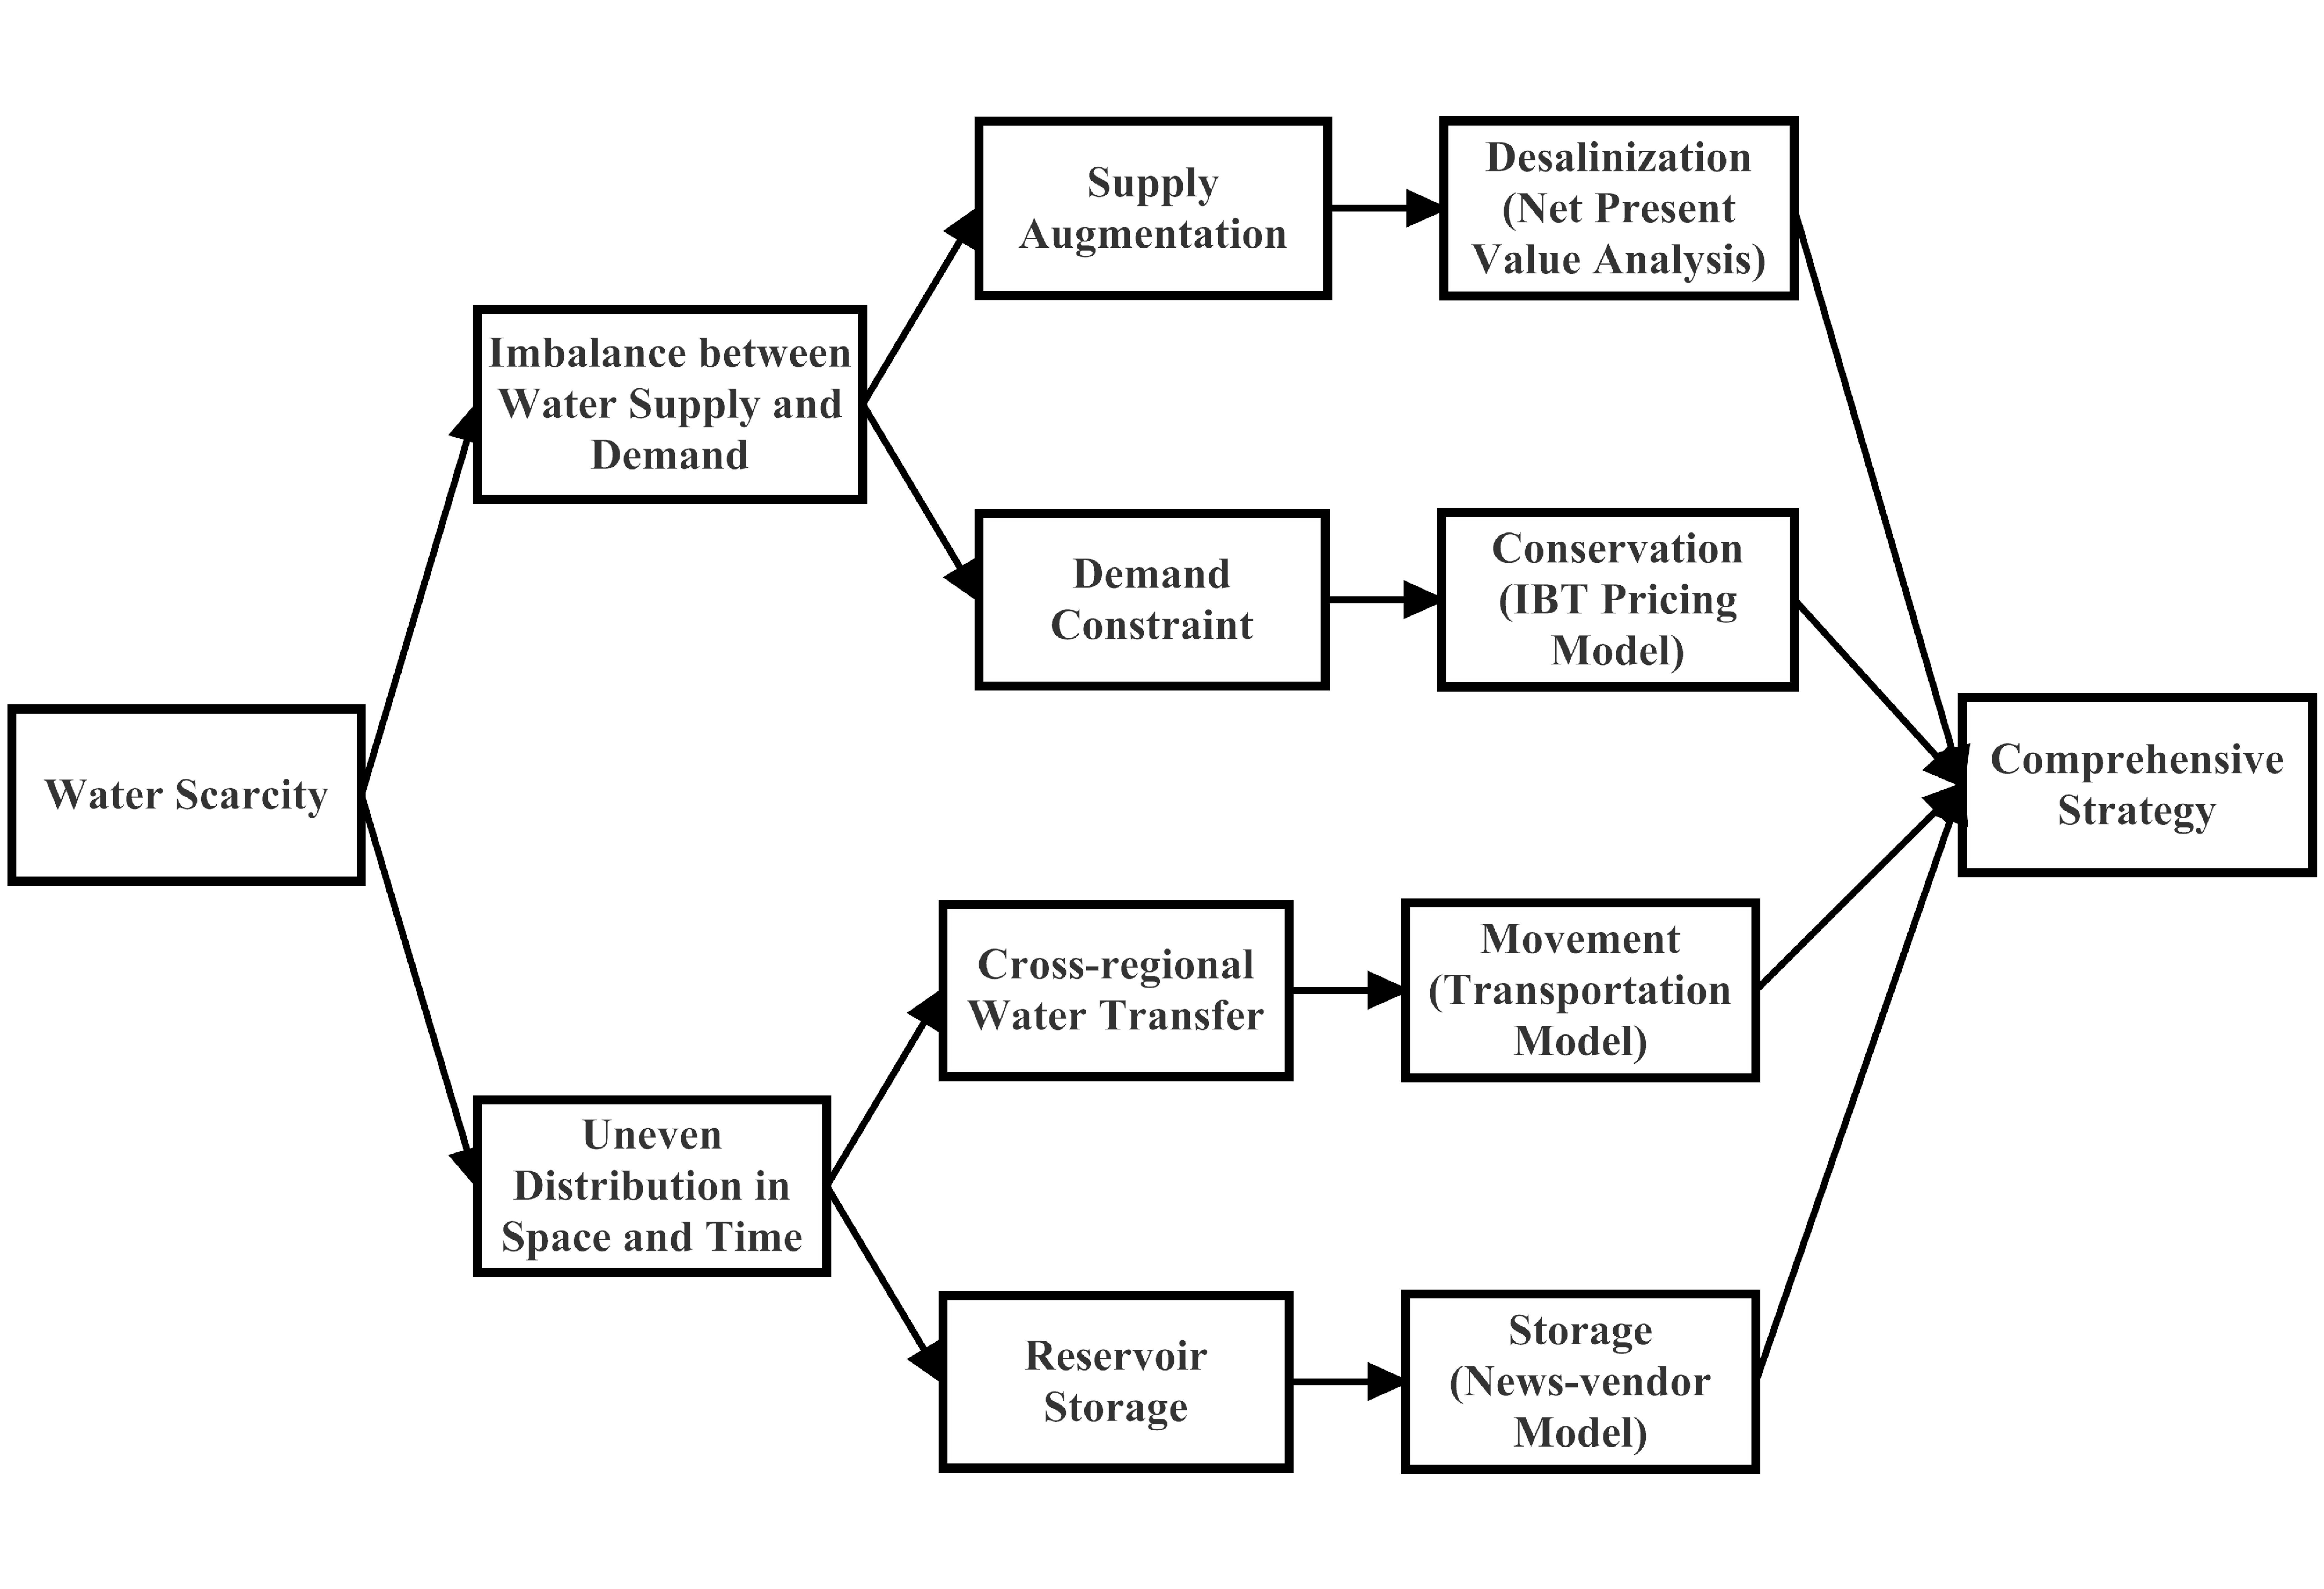
\includegraphics[width=12cm]{17444_figure_1}
\caption{Basic logic of our model} \label{mind}
\end{figure}
For the rest of our paper, we take every province in mainland China, as well as big municipalities like Beijing, into consideration. For simplicity, we will refer to all of them as "provinces" of China, and there are 30 provinces in our case. Hainan province, Hongkong SAR, Macao SAR and Taiwan district are omitted since they are more isolated to water management system of mainland China.

\section{Water Demand and Supply Prediction}
Many methods can be used to predict such time series data as water demand and supply, including auto regression, moving average, Box-Jenkins models, grey models, neural network and so on. As a superiority to conventional statistical models, grey models require only a limited amount of data to estimate the behavior of unknown systems\cite{Deng1989}\cite{Zhang2001}. Therefore, considering limited data available in China, we use a grey model to predict water demand and supply.

\subsection{Data Description}
The original province level data are adapted from 1999 to 2011 by National Bureau of Statistics of China\cite{NBS}.
\begin{itemize}
\item \textbf{We use ��water use (in $100$ million $m^3$)�� as water demand, including agriculture, industry, urban consumption and ecological protection.} Note that data for year 2004 data are unavailable due to unknown reasons. For consistency, we take the average demand of 2003 and 2005 to substitute for that of 2004.
\item \textbf{We use 40\% of total ��water resource(in $100$ million $m^3$)�� as water supply.} The total amount of water resource is the sum of surface water resources and groundwater resources less the overlap between the two. There are various hierarchies for the quality of natural water resources, a small portion of which is fresh water, and a even smaller portion of fresh water is available for us\cite{Dow2011}. Based on the statistics done by National Bureau of Statistics of China, we take an value of 40\% as the average portion of natural water resources as available for usage\cite{NBS}.
\end{itemize}

\subsection{The Grey Model}
We use GM(1,1) to predict the water demand and water supply in 2025. For every province, denote historical water demands and supplies by:
$$x^{(0)}=(x^{(0)}(1),x^{(0)}(2),\dots,x^{(0)}(13))$$
where $x^{(0)}(1)$ represents water demand or supply in 1999, and $x^{(0)}(13)$ represents historical data of water demand or supply in 2011. Under the rule of accumulated generation operation, we get
$$x^{(1)}=(x^{(1)}(1),x^{(1)}(2),...,x^{(1)}(13))
       =(x^{(1)}(1),x^{(1)}(1)+x^{(1)}(2),\dots,x^{(1)}(1)+\dots+x^{(1)}(13))$$
Averaging the sequence, we get a vector with 12 elemis:
$$ z^{(1)}=(z^{(1)}(2),z^{(1)}(3),\dots,z^{(1)}(13))$$
where $z^{(1)}(k)=\frac{x^{(1)}(k-1)+x^{(1)}(k)}{2},\ k=2,3,\dots,13.$ Next, establishing grey differential equation:
\begin{equation}
x^{(0)}(k)+az^{(1)}(k)=b,\ k=2,3,\dots,13
\label{e1}
\end{equation}
The corresponding albino differential equation for equation \ref{e1} is:
\begin{equation}
\frac{d x^{(1)}}{d t} +ax^{(1)}(t)=b
\label{e2}
\end{equation}
Solving the equation \ref{e2} yields:
$$ x^{(1)}(k+1)=(x^{(0)}(1)-\frac{b}{a})e^{-ak}+\frac{b}{a},\ k=1,2,\dots,12$$\
This method is given in the book \textit{Application of MATLAB in mathematical Modeling}\cite{Zhuo2011}.
After getting estimated demand and supply for each province in 2025, we calculate the water gap as:
\begin{center}
Gap = Supply - Demand
\end{center}

\subsection{Prediction Results}
\textbf{Figure \ref{figure1}} shows the results by running Matlab. Fifteen provinces will suffer from water shortage in 2025, namely Jiangsu, Xinjiang, Anhui, Shanghai, Henan, Hebei, Heilongjiang, Ningxia, Inner Mongolia, Gansu, Shanxi, Shandong, Hunan, Beijing and Tianjin, most of which are located in northern areas of China, except Shanghai and Hunan Province. The result is in agreement with the fact that water issue is more severe in northern China than in southern China, due to fewer precipitation, drier climate and more demand by agriculture, industry and urban consumption. More specifically, with additional $58.324$ billion $m^{3}$ needed, Jiangsu Province ranks top for water shortage, followed by Xinjiang Province and Anhui Province, with $36.05$ billion and $34.93$ billion respectively(see \textbf{Figure \ref{gb}}).\\
As can be seen in \textbf{Figure \ref{figure1}}, nearly half of China will be endangered by water shortage in 2025. Based on this prediction, in the following four sections, we propose four strategies to solve the problem. \\
\begin{figure}[htbp]
\centering
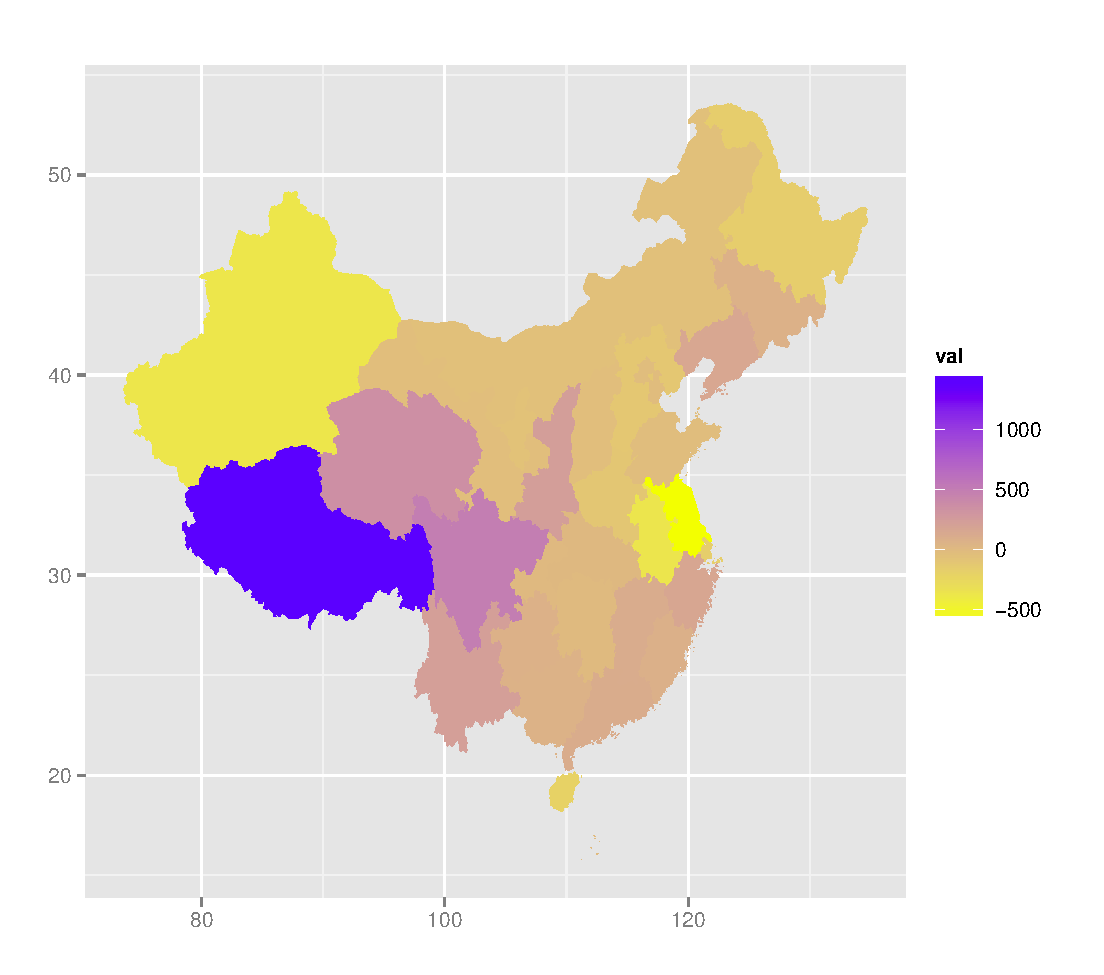
\includegraphics[width=12cm]{17444_figure_2}
\caption{\label{figure1}Gaps between demand and supply across China in 2025}
\end{figure}
\begin{figure}[htbp]
\centering
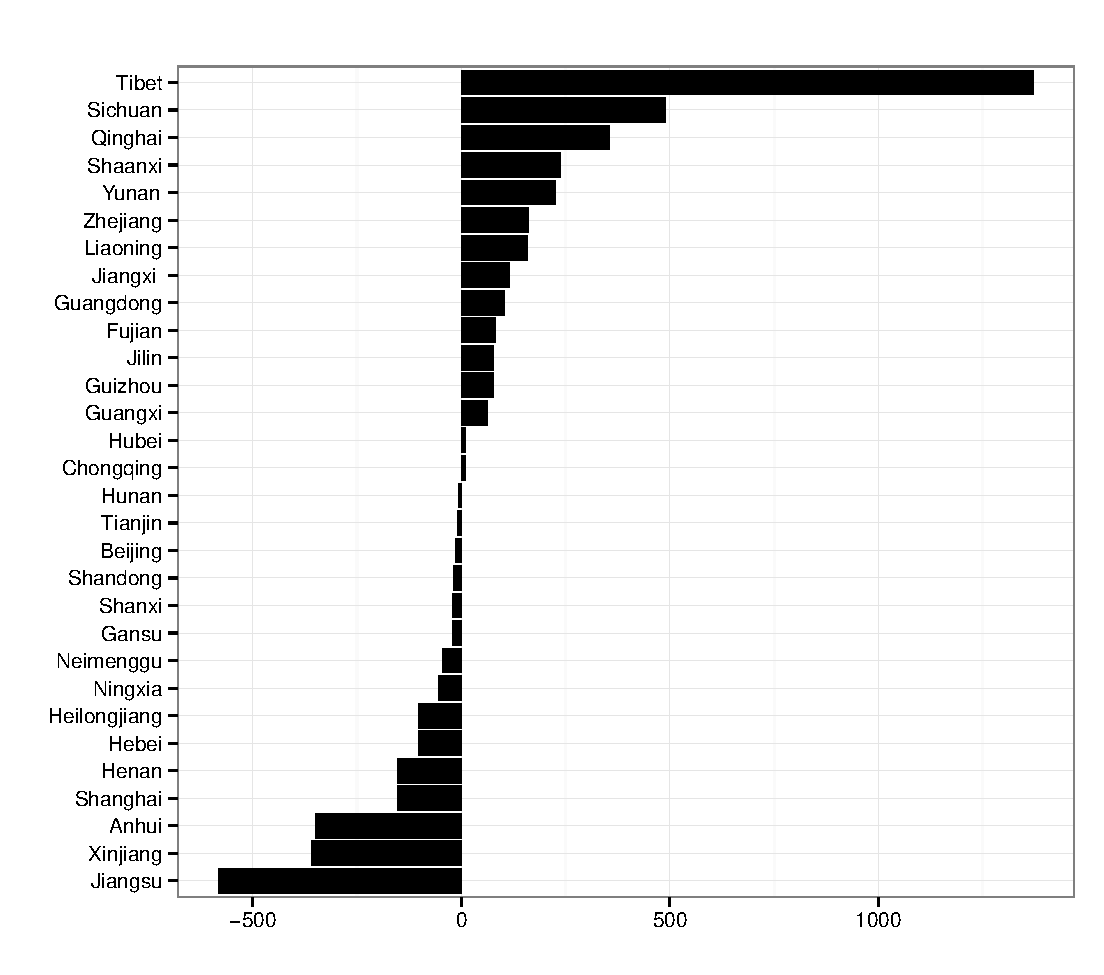
\includegraphics[width=12cm]{17444_figure_3}
\caption{\label{gb}Gaps between demand and supply across China in 2025}
\end{figure}

\subsection{Sensitivity Analysis}
In our assumptions, we mentioned that a portion (40\%) of water resources is available for usage. In this part, we try to test the model's sensitivity to changes in this number. \textbf{Figure \ref{AP}} illustrates results of the analysis. It is suggested by the figure that the change barely affects our predicted water distribution across the country. The value of water gaps, however, changes to some extent with different portions (absolute values of water gaps is shown by the legends in the figure).\\
\begin{figure}[htbp]
  \centering
  \subfigure[20\%]{\label{P20}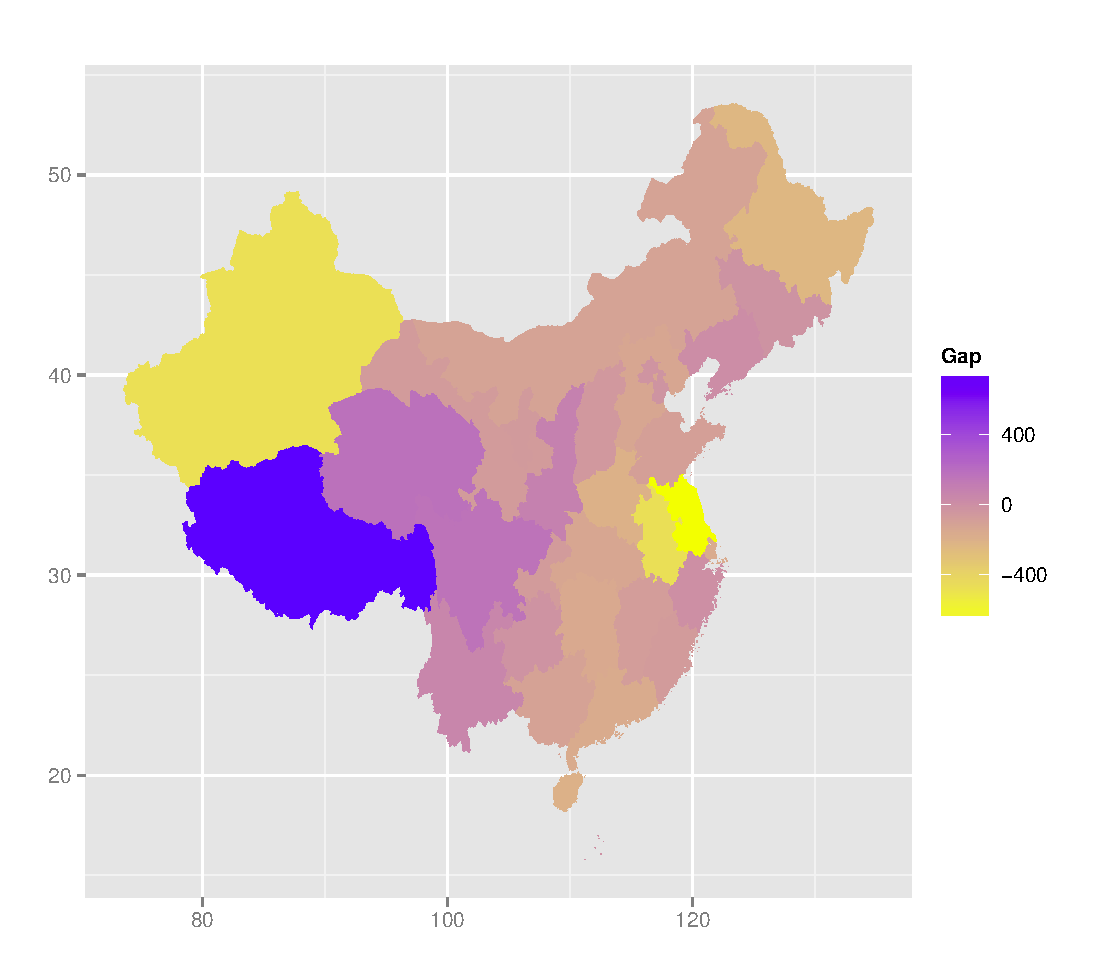
\includegraphics[width=6cm]{17444_figure_4_a}}
  \subfigure[60\%]{\label{P60}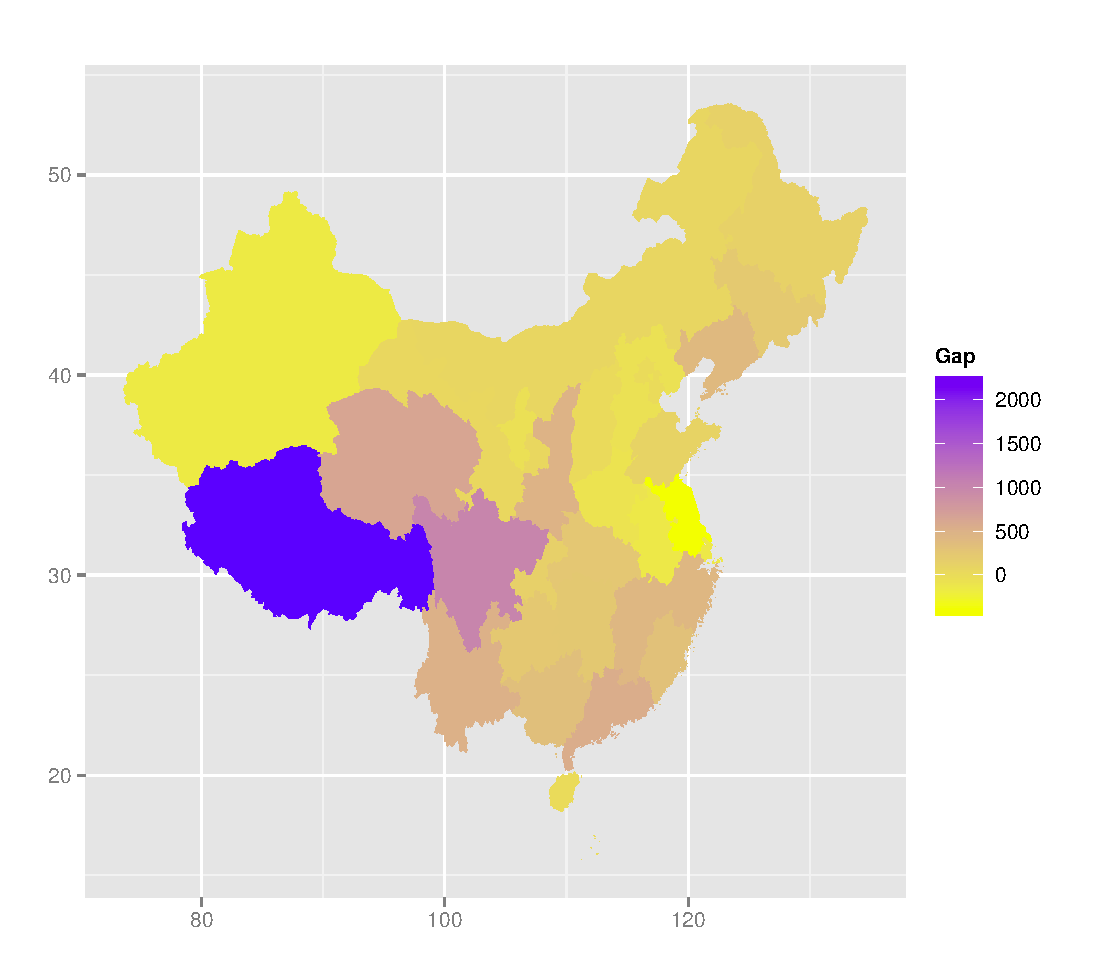
\includegraphics[width=6cm]{17444_figure_4_b}}
  \subfigure[80\%]{\label{P80}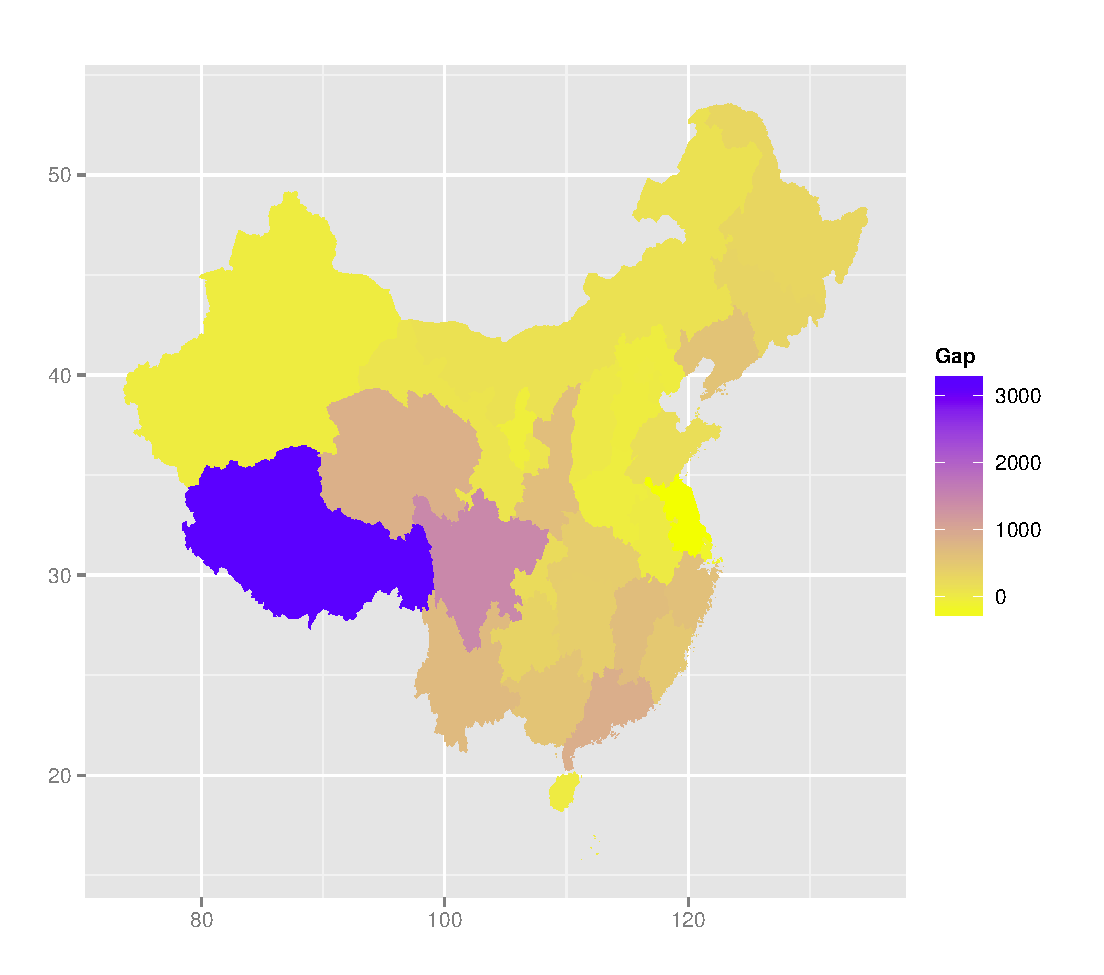
\includegraphics[width=6cm]{17444_figure_4_c}}
  \subfigure[100\%]{\label{P100}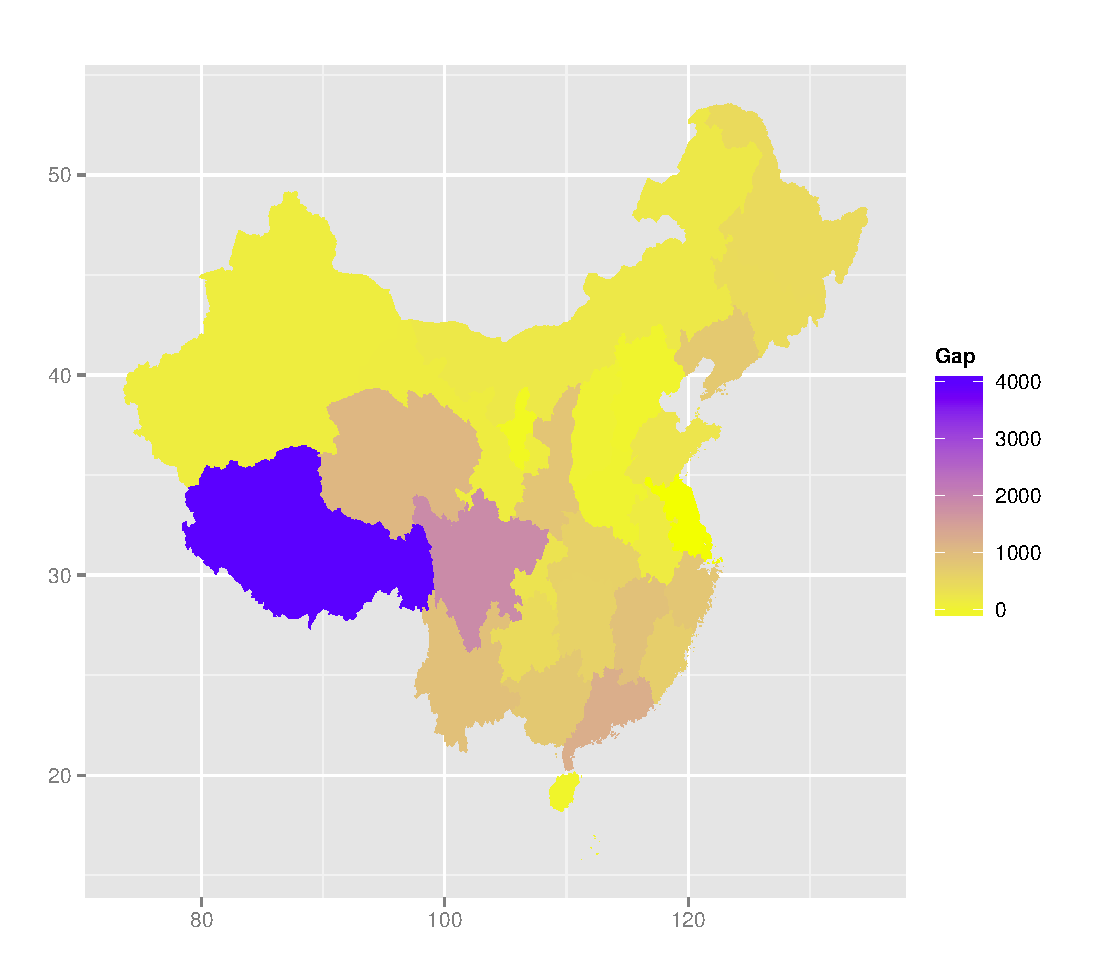
\includegraphics[width=6cm]{17444_figure_4_d}}
  \caption{Different water conditions using different portion of water supply}
  \label{AP}
\end{figure}
One flaw of the grey methods, as well as several models we mentioned before, is that we base the prediction on historical data trends and the assumption that this trend will continue in the future. It is never possible to accurately evaluate whether the assumption holds, so our model is still subject to possible error. A conceptual mode is offered by David et al. \cite{David1998}, which acknowledge the difficulty in quantifying water shortage prediction and base itself on dynamic system of water supply and demand and only requires a set of data in one single year. The authors discussed the precision of the model in their report. However, due to lack of required data, we give up on using their model. When related data are available, we suggest considering their model. More issues of data precision are discussed in the part of strengths and weaknesses of model.

\section{Strategy 1: Water Transfer}
Given the estimated water conditions in 2025, we use a mathematical model to come up with a strategy for water transfer.\\
There are several major rivers in mainland China, and scholars often partition China into regions around these rivers.
These regions are often referred to "river basins". An illustration of this partition is shown in \textbf{Figure \ref{regions1}}. For simplicity, we refer to river basins as "regions" for the rest of this part. \\
Since water transportation within a region is relatively easy and costless compared to across regions, we now only consider water transportation across regions.
That is, we calculate water gap of every region by summing up that of every province belonging to the region.\\
Firstly, for every region, we take its water supply and demand as given, and figure out a model to determine an optimal transportation strategy satisfying the demand of every province.  Based on this model, we input related data and get the desired strategy.
\begin{figure}[htbp]
\centering
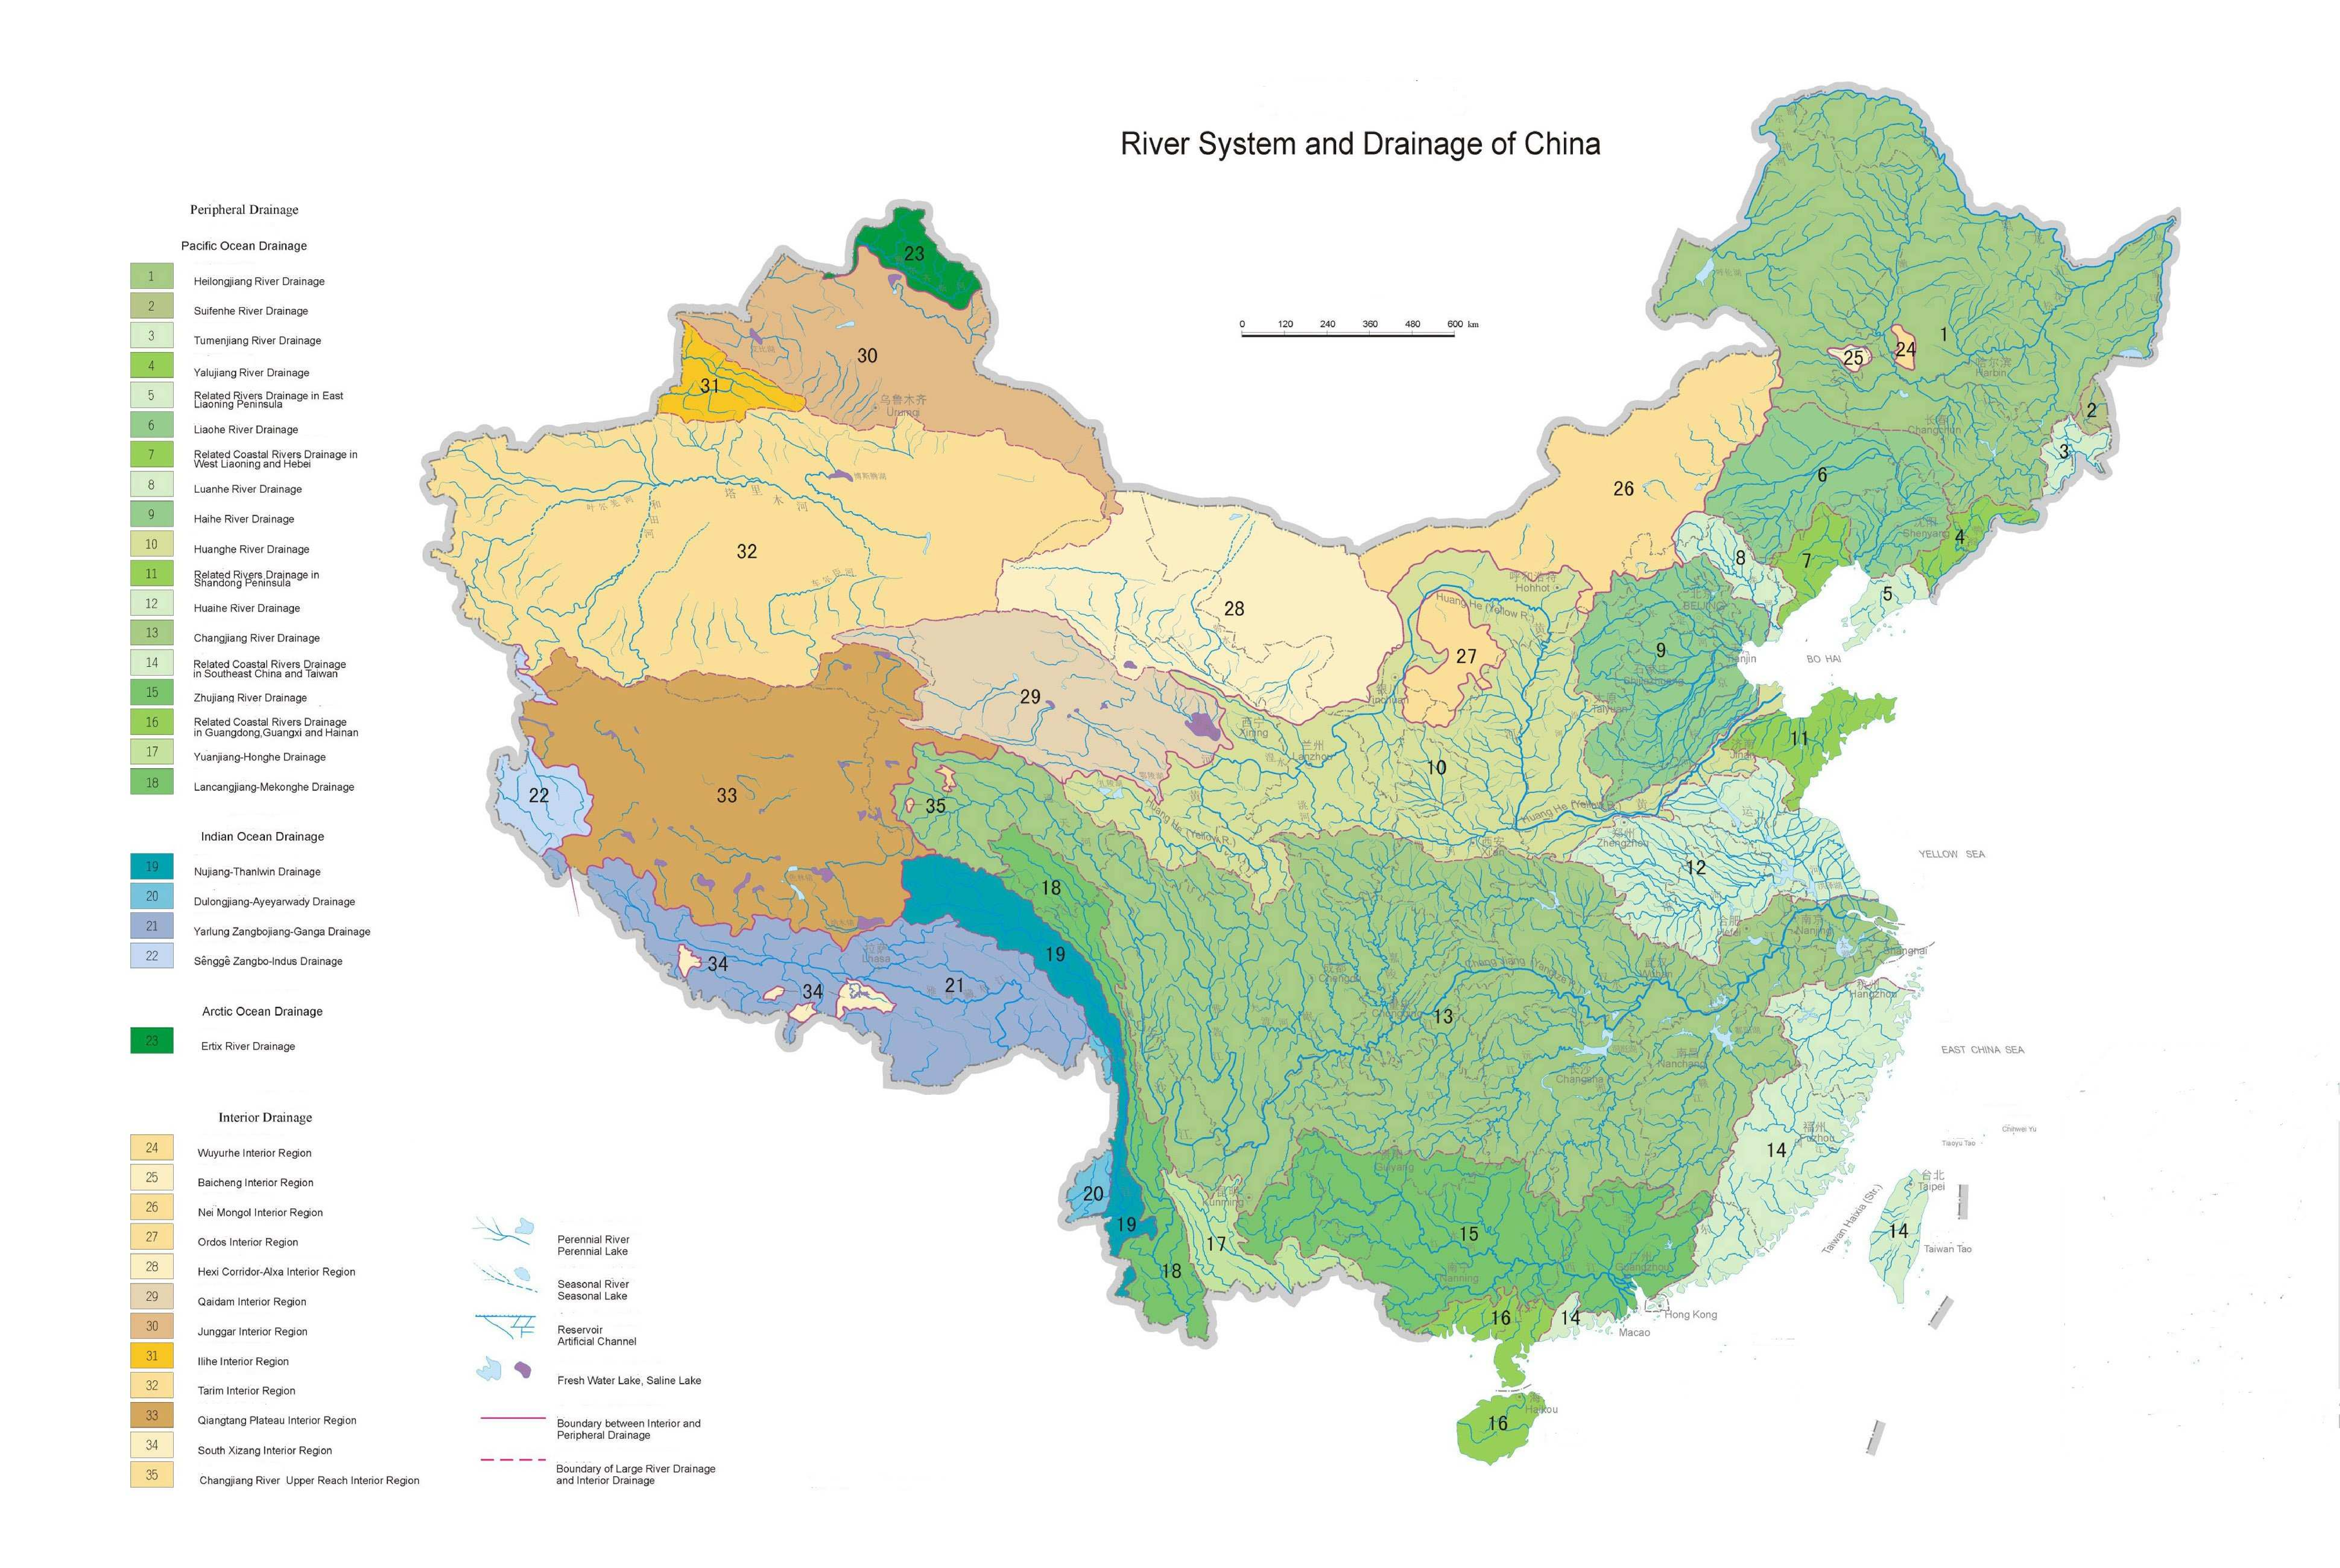
\includegraphics[width=12cm]{17444_figure_5}
\caption{\label{regions1}An illustration of river basins in China. Source: \textit{Atlas of Natural Disaster System of China}, published by \textit{Science Press} in 2003}
\end{figure}

\subsection{Assumptions}
\begin{itemize}
\item \textbf{Cost of transportation is proportional to the volume and the distance of water transported.} That is, the more and the longer distance water is transported , the more it costs for the government. It is unrealistic to transport a very small amount of water across regions, so we assume that the volume of water transported is large enough to ignore economies of scale.
    %Explanation: We regard a small volume of transportation as reasonable in spite that in reality such transportation might cost much but have little effect.
\item \textbf{Transportation is accomplished at the beginning of a year.} We simplify a continuous water transfer to an event accomplished at the beginning of a year. After transportation, water demands in China are met to the largest extent.
\item \textbf{There exists a water transportation channel (or other water transfer projects) between every pair of regions.} There are several cross-regional water transfer projects built in China. A famous example is the South-North Water Transfer Project. We assume that under the help of these water transfer projects we are able to transport water between regions.
\end{itemize}

\subsection{Notations}
\begin{itemize}
    \item $R_i$: Region i. There are at total M regions involved. \\
    \item $s_i$: Water supply of region i at the beginning of a year. \\
    \item $d_i$: Water demand of region i for the year. \\
    \item $g_i=s_i-d_i$: Water gap of region i. \\
    \item $c_{ij}$: Cost of transportation for per unit of water from region i to region j. \\
    \item $E$: The set of net water suppliers, i.e., regions with water excess. \\
    \item $S$: The set of net water demanders,i.e., regions with water shortage. \\
    \item $m$: Number of elements in E, i.e., number of net water suppliers. \\
    \item $n$: Number of elements in S, i.e., number of net water demanders. \\
    \item $x_{ij}$: The volume of water transported from region i to region j.\\
    \item $C$: Total cost of water transportation.\\
\end{itemize}

\subsection{The Transportation Model}
We first decide upon the set of regions with water excess or shortage by checking their gaps $g_i$'s. We let $R_i\in E$ if $g_i>0$ and let $R_i\in S$ if $g_i<0$.
For legibility, we rename a positive gap from $g_i$ to $a_i$ and negative ones from $g_i$ to $b_i$. We discuss below different cases corresponding to different values of $G=\sum_{i=i}^Mg_i$.\\
\paragraph{In the case of $G=0$, total water excess equals to total water shortage.} The optimization problem can be listed as follows:\\
$$\min C=\sum_{i=1}^m\sum_{j=1}^nc_{ij}x_{ij}$$
\[
\rm{s.t.}\begin{cases} \sum_{j=1}^nx_{ij}=a_i,\ (i=1,2,\dots,m) &\text{(Region $i$ supplies
water of volume $a_i$)}\\
\sum_{i=1}^nx_{ij}=b_j,\ (j=1,2,\dots,n) &\text{(Region $j$ demands water of volume $b_j$)}\\
x_{ij}\geq0,\ (i=1,2,\dots,m; j=1,2,\dots,n) &\text{(Nonnegative constraints)}
\end{cases}
\]
\paragraph{In the case of $G>0$, total water supply exceeds total water demand.} Therefore, everything
else being equal, the first constraint changes to:$$\sum_{j=1}^nx_{ij} \leq a_i,\ (i=1,2,\dots,m)$$\\
\paragraph{In the case of $G<0$, total water demand cannot be satisfied by water supplies inside the
country.} Therefore the second constraint changes to: $$\sum_{i=1}^nx_{ij} \geq b_j,\ (j=1,2,\dots,n)$$\\

\subsection{Solution}
\subsubsection{Parameter estimation}
\paragraph{Regions.} As is shown in \textbf{Figure \ref{regions2}}, we use one of the mainstream partitions which divides mainland China into 7 major regions. We specify them in the \textbf{Table \ref{regions3}} below.
\begin{figure}[htbp]
\centering
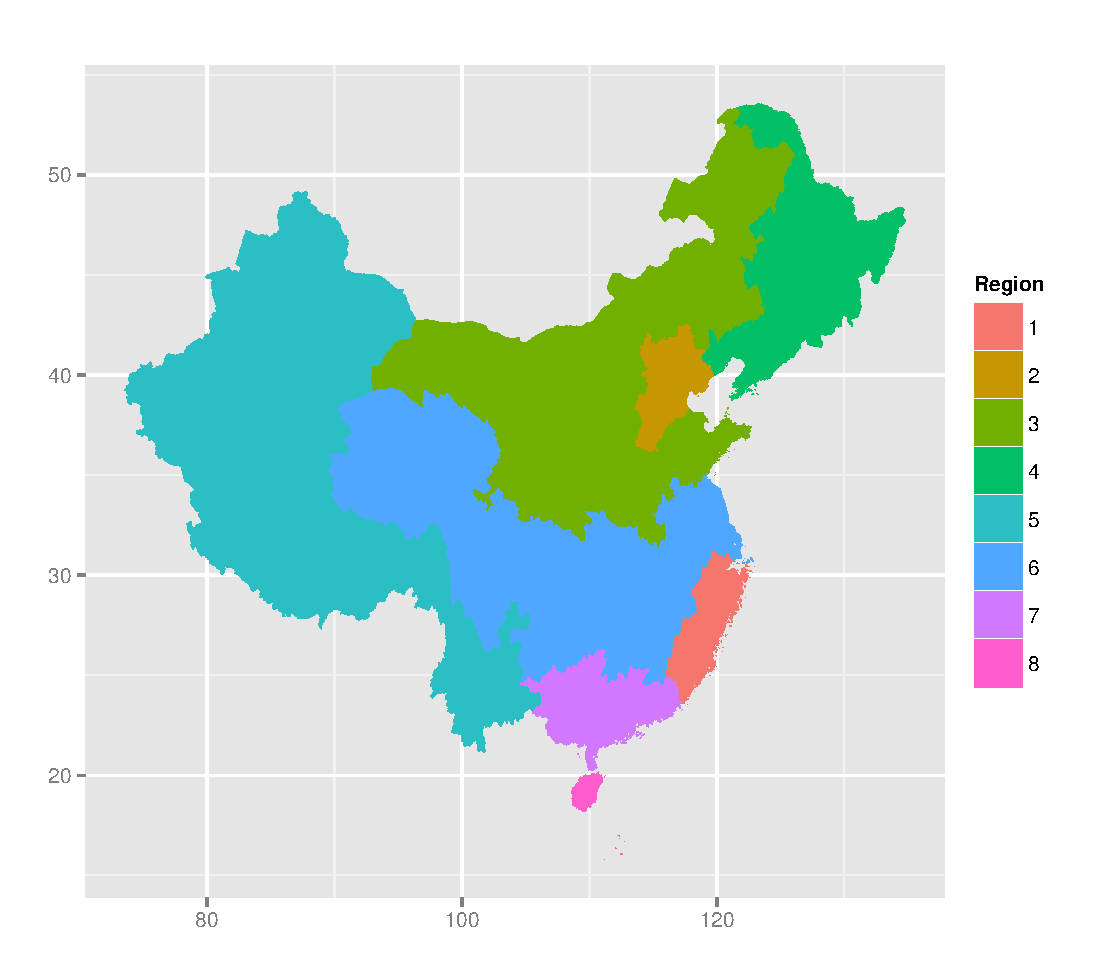
\includegraphics[width=12cm]{17444_figure_6}
\caption{\label{regions2}The 7 regions we use in our model (Note that the $8^{th}$ region in the graph is Hainan Province, which we ignore in our model.)}
\end{figure}
% Table generated by Excel2LaTeX from sheet 'Sheet1'
\begin{table}[htbp]
  \centering
  \caption{Classification of provinces}
    \begin{tabular}{rll}
    \toprule
    Notation & River Basin & Provinces \\
    \midrule
    $R_1$    & The Southeast River Basin & Fujian, Zhejiang; \\
    $R_2$    & The Haihe River Basin & Beijing, Hebei, Tianjin; \\
    $R_3$    & The Yellow River River Basin & Gansu, Henan, Inner Mongolia,\\ &&Ningxia, Shaanxi, Shandong, Shanxi; \\
    $R_4$    & The Songliao River Basin & Heilongjiang, Jilin, Liaoning; \\
    $R_5$    & The Southwest River Basin & Tibet, Xinjiang, Yunnan; \\
    $R_6$    & The Long River River Basin & Anhui, Chongqing, Guizhou, Hubei,\\&& Hunan, Jiangxi, Jiangsu, Qinghai,\\&& Shanghai, Sichuan; \\
    $R_7$    & The Perl River River Basin & Guangdong, Guangxi \\
    \bottomrule
    \end{tabular}%
  \label{regions3}%
\end{table}%

\paragraph{Supplies and demands.} We get from part 1 the projected water condition in 2025. According to our estimation, two regions will face water shortage, namely $R_2$ (12.32 billion $m^3$) and $R_3$(5.21 billion $m^3$), and the rest 5 regions have water surplus (26.18 billion $m^3$ for $R_1$, 15.90 billion $m^3$ for $R_4$, 128.68 billion $m^3$ for $R_5$, 53.37 billion $m^3$ for $R_6$, 19.70 billion $m^3$ $R_7$). Total water gap in China will sum up to $G$=179.27 billion $m^3$. The net supplies and demands are also available, using data above.\\
In this case, we have $E=\{R_1,\ R_4,\ R_5,\ R_6,\ R_7\}$, and $S=\{R_2,\ R_3\}$.
\paragraph{Cost of transportation per $m^3$ per $km$.} We first determine the distances between regions. Since shapes of regions are irregular, there is no way to accurately capture the intrinsic distances, which leaves us to estimate such values. We take mean distance between provinces of each region as a measurement of region distances. To approximate this measurement, we choose a central city in each region and take the distance between these cities. We take cities Wenzhou, Beijing, Yan'an, Changchun, Lasa, Chongqing and Foshan to represent the center of from $R_1$ to $R_7$, respectively (see \textbf{Figure \ref{network}}). The distances calculated are listed below in \textbf{Table \ref{distance}}. For example, the element in the first row and the first column stands for the distance between $R_1$ and $R_2$.  We arbitrarily assume that transporting water 1 km costs 0.1 yuan, then the unit cost equals to 10\% of the distance between regions involved.\\
\begin{figure}[htbp]
\centering
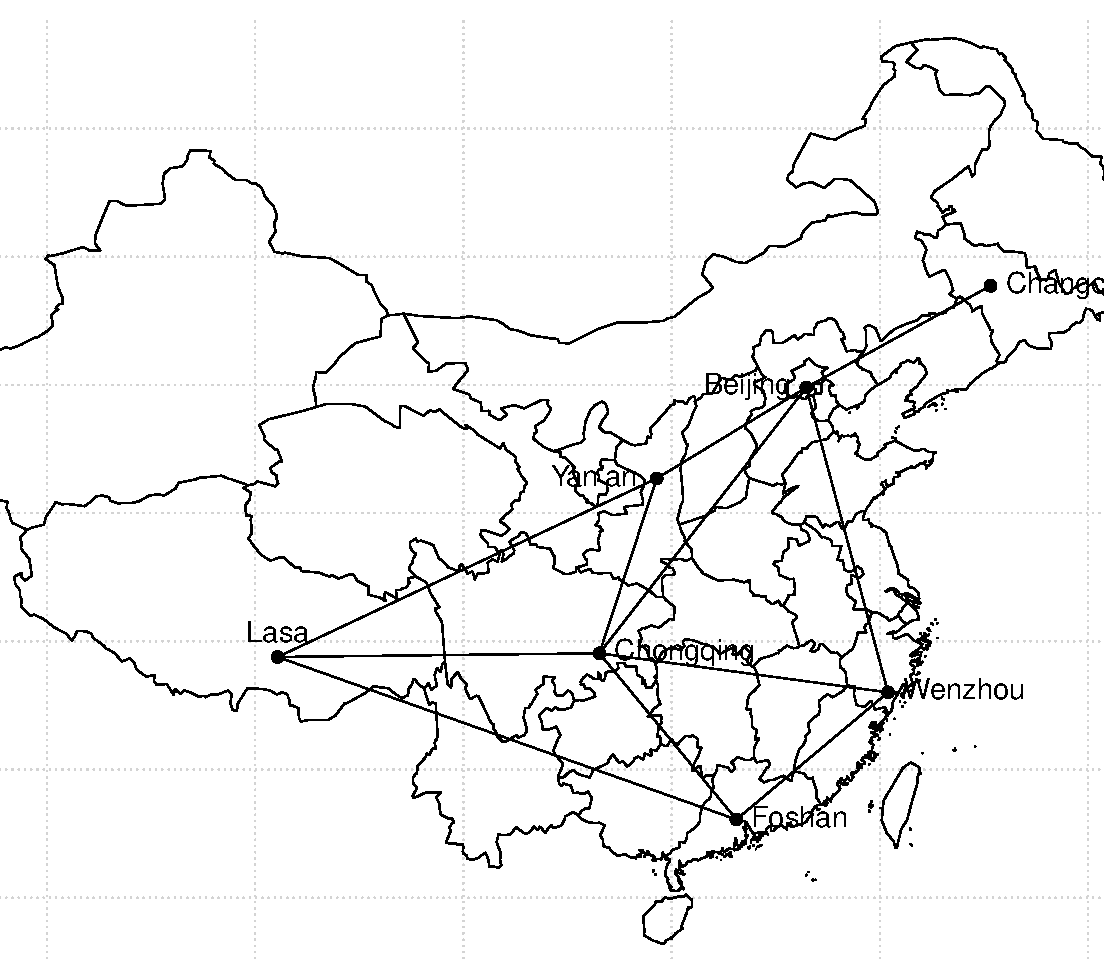
\includegraphics[width=12cm]{17444_figure_7}
\caption{\label{network}Cities standing for centers for regions and an illustration of water transportation network}
\end{figure}
% Table generated by Excel2LaTeX from sheet 'Tabelle1'
\begin{table}[htbp]
  \centering
  \caption{Distance matrix for regions}
    \begin{tabular}{rrrrrrr}
    \toprule
          & $R_1$    & $R_2$    & $R_3$    & $R_4$    & $R_5$    & $R_6$ \\
    \midrule
    $R_2$ & 1382  &       &       &       &       &  \\
    $R_3$ & 1420  & 710   &       &       &       &  \\
    $R_4$ & 1809  & 858   & 1564  &       &       &  \\
    $R_5$ & 2880  & 2564  & 1872  & 3400  &       &  \\
    $R_6$ & 1390  & 1460  & 828   & 2300  & 1490  &  \\
    $R_7$ & 940   & 1904  & 1550  & 2570  & 2310  & 980 \\
    \bottomrule
    \end{tabular}%
  \label{distance}%
\end{table}%
The problem is a linear programming problem, or more, a typical transportation model. With costs, supplies and demands available, we specify the model and solve for the problem. The result is shown in \textbf{Table \ref{Tsolution}}.\\

\subsubsection{Conclusion}
Based on the solution given by solving for the problem, we have a transportation strategy to deal with water shortage in the year of 2025:\\
Transport 12.32 billion $m^3$ water from $R_4$ (The Songliao River Basin) to $R_2$ (The Hehai River Basin), which costs 1057.30 billion yuan;\\
transport 5.21 billion $m^3$ water from $R_6$ (The Long River River Basin) to $R_3$ (The Yellow River River Basin), which costs 431.46 billion yuan.\\
The total cost sums up to 14.88 billion yuan;
% Table generated by Excel2LaTeX from sheet 'Sheet2'
\begin{table}[htbp]
  \centering
  \caption{Water transportation strategy}
    \begin{tabular}{cccc}
    \toprule
    From  & To    & Volume & Cost \\
    \midrule
    $R_4$    & $R_2$    & 12.32 & 1057.30 \\
    $R_6$   & $R_3$    & 5.21  & 431.46 \\
          &       & Total Cost      & 1488.76 \\
    \bottomrule
    \end{tabular}%
  \label{Tsolution}%
\end{table}%

\subsection{Sensitivity Analysis}
The model uses a lot of estimated data as parameters, in addition to the estimated water gaps given by the prediction model. Therefore, we should carefully examine the model's sensitivity to changes in our estimation. Using the data given above as a basis, we look into the effect of partial changes of data. From \textbf{Table \ref{A2}} we see that the total cost does not change more than estimation. But still, our model is to some extent reliant on the values of estimations. However, the optimality of our result is not negated by this sensitivity, since the model yields an analytic optimal result. In other words, our model always produces the best transportation path given that the related data are correct.
% Table generated by Excel2LaTeX from sheet 'Sheet1'
\begin{table}[htbp]
  \centering
  \caption{Sensitivity analysis of the transportation model}
    \begin{tabular}{cc}
    \toprule
    Changes in distance between $R_2$ and $R_4$  & Change in total cost \\
    \midrule
    20.00\% & 14.20\% \\
    10.00\% & 7.10\% \\
    -10.00\% & -7.10\% \\
    -20.00\% & -14.20\% \\
    \bottomrule
    \end{tabular}%
  \label{A2}%
\end{table}%

\section{Strategy 2: Water Storage}
Unlike water transfer, water storage is mainly used to deal with uneven water distribution in time, in which case water is stored for later use. Methods range from natural water stores, such as groundwater aquifers, to reservoirs behind major dams. In this section, we examine how reservoirs can be best used to resolve the future shortage.\\
How much water do we need for later use is similar to a stock problem, which determines an optimal order quantity at a certain time point to satisfy the stochastic demands in the future. Therefore, we apply classic news-vendor model to solve the problem. For the convenience of modeling, we refer $"demand"$ to water gaps derived above. \\

\subsection{Assumptions}
\begin{itemize}
\item \textbf{Reservoirs store water from both its upstream and precipitation.} These are two main water sources for reservoirs. The order quantity from its upstream should exclude precipitation;
\item \textbf{Reservoirs store water to satisfy local and downstream demands}. It is impossible or too expensive for reservoirs to transport water to the areas upstream. The amount needed equals to demand less normal storage, which is the existing storage in the reservoir;
\item \textbf{We allow stock-out costs and holding costs to occur}. In the former case, areas in the downstream suffer from water shortage, thus incurring economic loss. In the latter case, excess water lead to opportunity cost lost by upstream areas;
\item \textbf{Downstream demands are normally distributed,} whose cumulative distribution function is $F(x)$ and probability density function is $f(x)$.
\end{itemize}

\subsection{Notations}
\begin{itemize}
\item $r$: Downstream demand, which is stochastic. \\
 \item   $q$: Order quantity by reservoir \\
 \item   $s$: Stock-out cost, reflected by the economic loss in the downstream when gaps cannot be met. \\
   \item $c$: Holding cost, reflected by the opportunity cost lost in the upstream when order quantity exceed gaps. \\
   \item $TC$: Total cost for the whole system. \\
\end{itemize}

\subsection{The Stock Model: The News-vendor Problem}
We aim to determine optimal order quantity to minimize the total cost. So the target function can be written as follows:
$$
\rm{min}\ TC(q)=\int_0^q c(q-r)f(r)dr +\int_q^\infty s(r-q)f(r)dr,
\rm{s.t} \ q \geq 0
$$
To solve the problem, we set the first order derivative of $TC(q)$ qual to zero and get:
\begin{equation}
\frac{d TC(q)}{d q}=c\int_0^q f(r)dr-s\int_q^\infty f(r)dr=0
\label{e3}
\end{equation}
Taking the second-order derivative of $TC(q)$,we find that:
$$\frac{d^{2}TC(q)}{d q^{2}}=(c+s)f(q)\geq0$$
So, the optimal solution exists for the problem. Solving the equation \ref{e3}, we get the optimal order quantity when:
\[
\frac{\int_0^q f(r)dr}{\int_q^\infty f(r)dr}=\frac{s}{c}
\]

\subsection{Case Study}
We apply theoretical model to the \textit{Three Gorges Reservoir}, which is the largest reservoir in China. Located in Yichang city and spanning the Yangtze River, the \textit{Three Gorges Reservoir} is the main water supplier to its downstream areas, including provinces Jiangsu, Anhui, Shanghai and Hunan. Both the representativeness and the strategic significance lead us to use the \textit{Three Gorges Reservoir} as a case to study.\\
\subsubsection{Normality Test for Historic Demands}
We take historical data of total water demands of provinces around the downstream of The Three Gorges Reservoir to test our assumption of their normality. Q-Q plot of data (see \textbf{Figure \ref{qqp}}) suggests that they behave quite well in terms of normality. A Shapiro-Wilk test also confirms our hypothesis(W = 0.9885, p = 0.5429), which means that under the hypothesis of normalities of sample data, the possibility of getting a W statistic more extreme than or as extreme as the observed one (W = 0.9885) is 54.29\%. Therefore, our data supports the hypothesis and we accept the normality assumption.\\
\begin{figure}[h]
\small
\centering
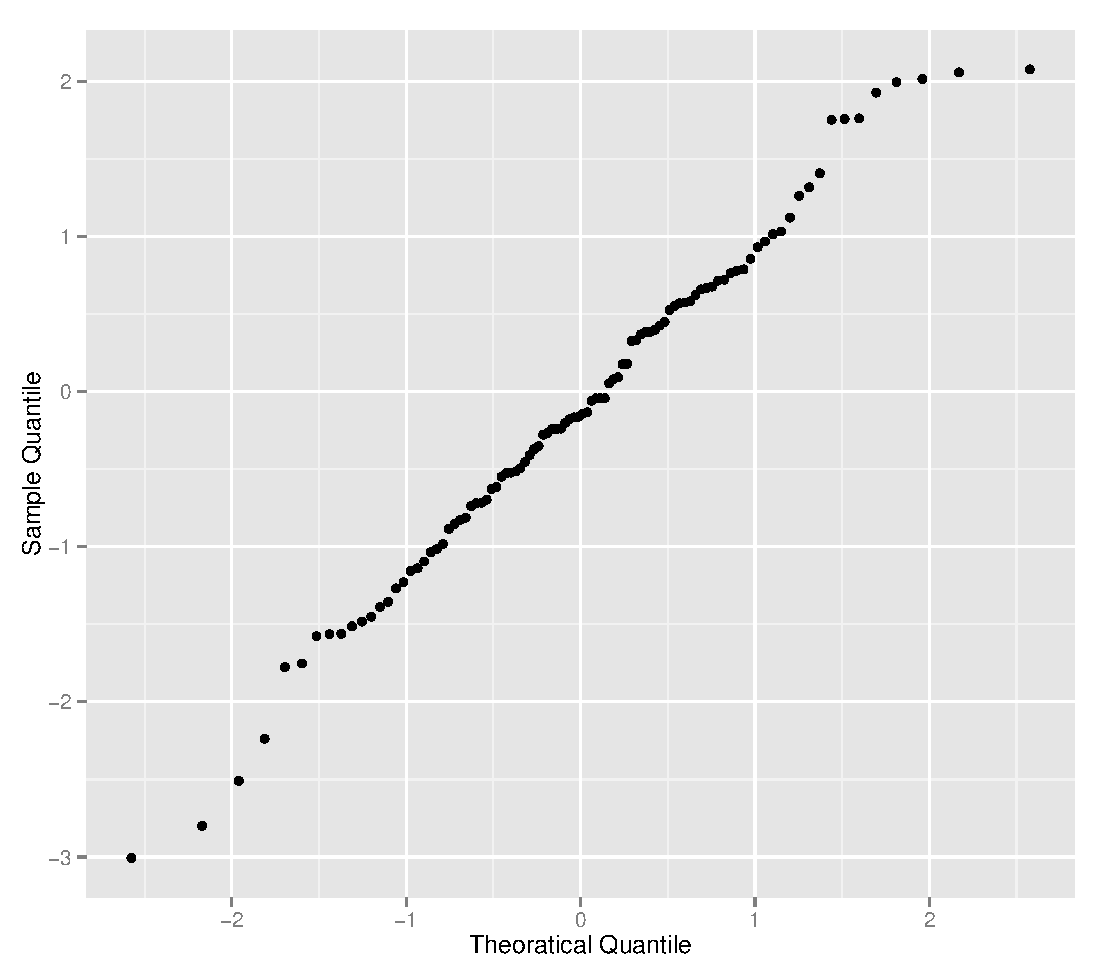
\includegraphics[width=12cm]{17444_figure_8}
\caption{Q-Q plot of historical data} \label{qqp}
\end{figure}

\subsubsection{Parameters Estimation}
We define the stock-out cost as economic loss suffered by downstream areas due to inadequate water, since water shortage has a direct negative impact on agricultural production, industrial output and urban consumption, further influencing the local GDP. Water consumption per 10 thousand yuan GDP is an official method to measure the contribution of water to the total GDP. So we use how much GDP can 1 $m^3$ water generate to quantify the stock-out cost. \\
We define holding cost as the opportunity cost under which upstream areas can use those excess water for other use, again, such as agricultural production, industrial output and urban consumption. Accordingly, we also use how much GDP can $1$ $m^3$ of water generate to quantify the holding cost. We ignore negative environmental effects for simplicity.\\
As for the Three Gorges Reservoir, its downstream areas include Hubei Province, Hunan Province, Jiangxi Province, Anhui Province and Shanghai and its upstream areas include Qinghai Province, Sichuan Province, Guizhou Province and Chongqing. Stock-out cost of each province is calculated by local GDP dividing water consumption, and the total stock-out cost,denoted by $s$,is the average of that in its downstream area. So is the case with the total holding cost,denoted by $c$. Original data are adapted from National Bureau of Statistics \cite{NBS} and through simple computation, we get $s=53.44\ \rm{yuan}/m^{3}$ and $c=222.43\ \rm{yuan}/m^{3}$.\\
Taking into account the precipitation and normal storage in the reservoir,which is the minimal requirement of the reservoir, we define net demand as:
\begin{center}
Net demand = Gap - Precipitation -Normal Storage
\end{center}
 Gap is the average of respective provinces in downstream or upstream,which equals to 154.48 billion $m^{3}$.
Precipitation is calculated by:
\begin{center}
Precipitation = Annual precipitation in Yichang city $\times$ Surface area of Three Gorges Reservoir
            = $1.138 \times 1525 \times 10^{7} = 17.4\ \rm{million}\ m^{3}$
\end{center}
where data are adapted from Wikipedia, from which we also get the normal storage of 393 $m^{3}$.\\
So we can get the net demand of 115.16 billion $m^{3}$. Since we treat precipitation and normal storage as constants, standard deviation of net demand equals to that of gap, i.e., 440.\\
\subsubsection{Results for the Theoretical Model and Simulation}
With known normal distribution of net demand and parameters of $s$ and $c$, we can solve the news-vendor problem theoretically. The optimal order quantity is 84.1 billion $m^{3}$, which is clearly exhibited in \textbf{Figure \ref{sn}}.  We use the Matlab symbolic computational methods to come up with the expected total cost of every possible order quantity. From the \textbf{Figure \ref{tf}}, the best order quantify of 84.1 trillion $m^3$ is apparent. We randomly generate 500 random water demand of downstream of Three Georges Dam,  according to a Gaussian Distribution (mean = 1152, standard deviation = 440) and then compute the total cost given the optimal order quantity 84.1 trillion $m^3$ (see \textbf{Figure \ref{simu}}).
\begin{figure}[htbp]
\centering
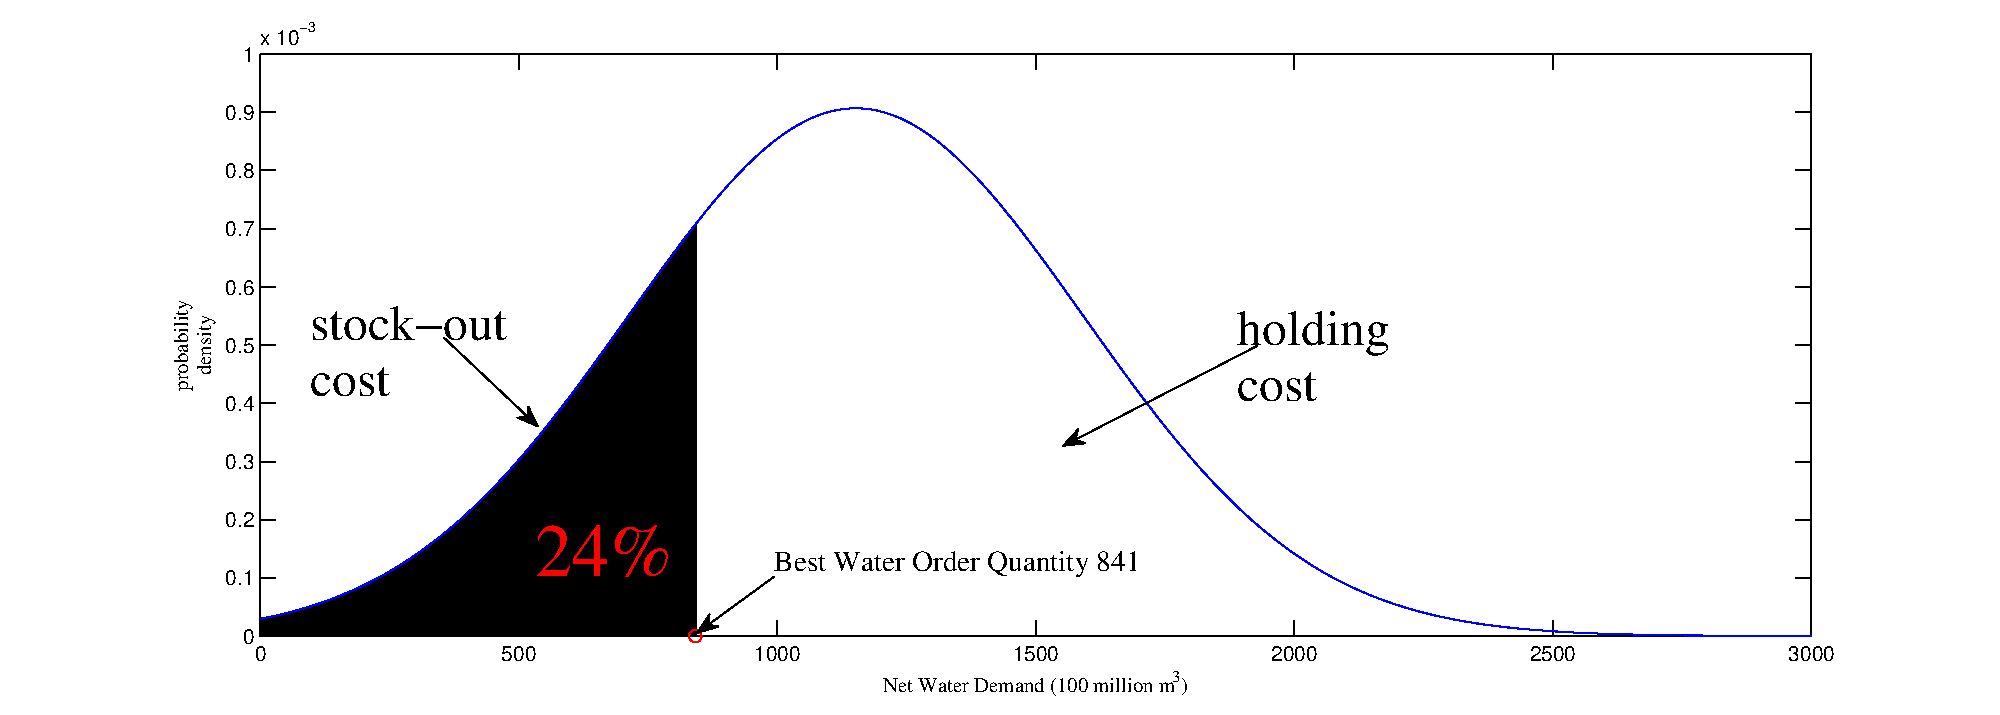
\includegraphics[width=15cm]{17444_figure_9}
\caption{\label{sn}Solution to the news-vendor model}
\end{figure}
\begin{figure}[htbp]
\centering
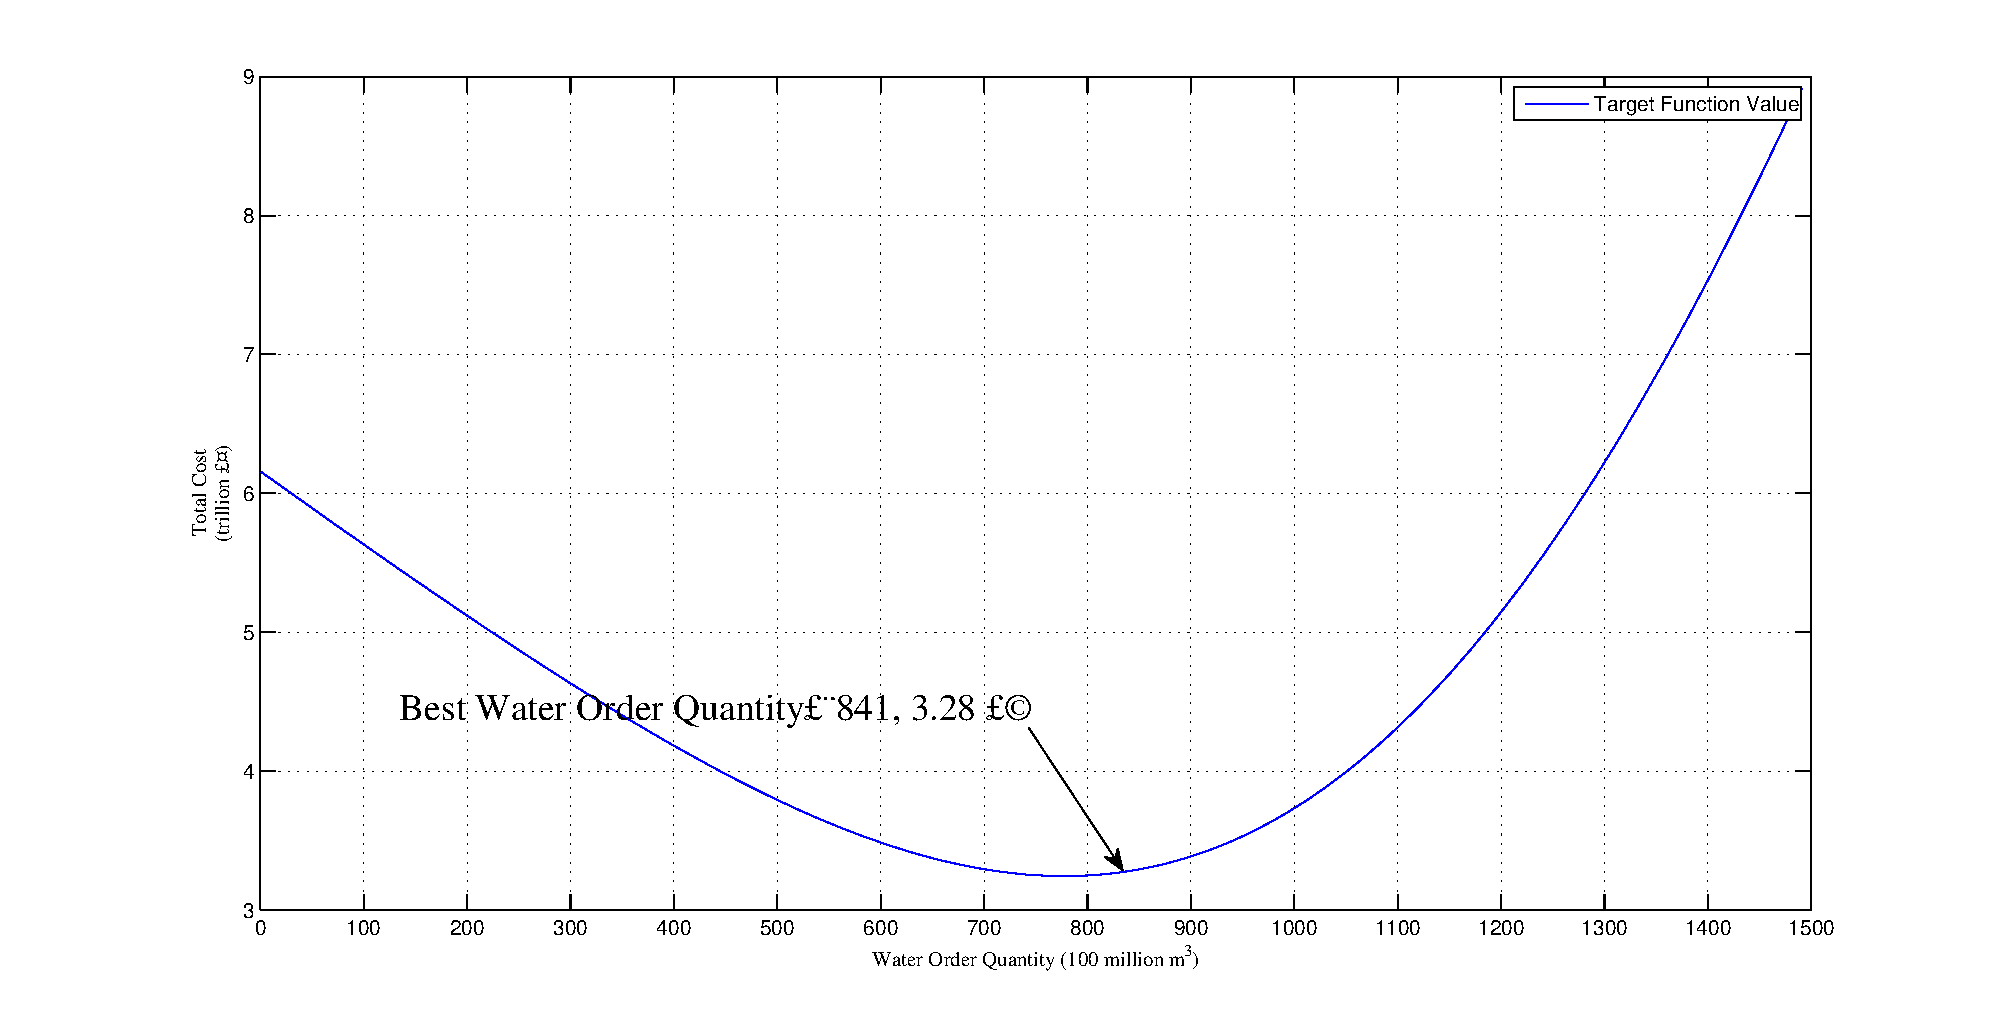
\includegraphics[width=15cm]{17444_figure_10}
\caption{\label{tf}Target function}
\end{figure}
\begin{figure}[htbp]
\centering
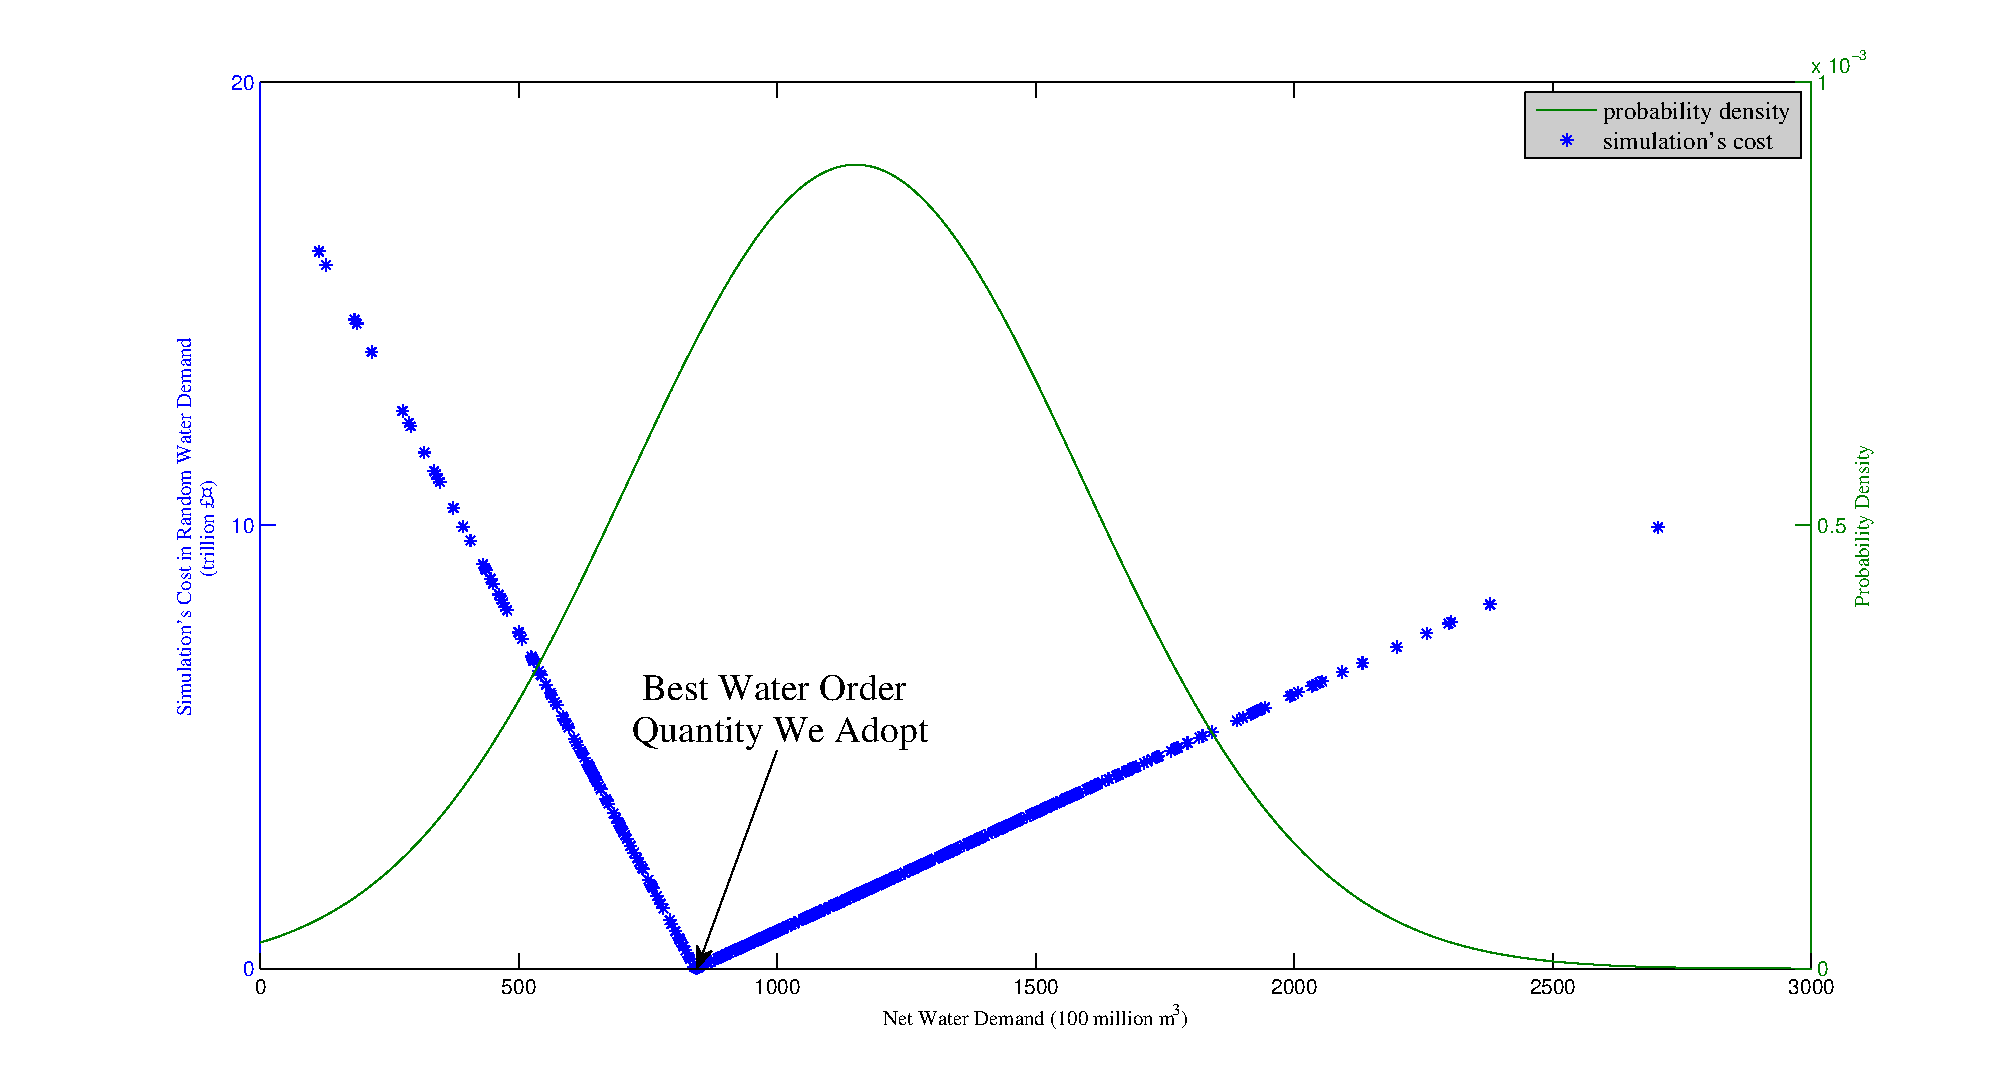
\includegraphics[width=15cm]{17444_figure_11}
\caption{\label{simu}Monte-Carlo simulation of water demands}
\end{figure}

\subsubsection{Strategy}
Considering 2025 as the next stock period, we suggest that Three Gorges Reservoir store 84.1 billion $m^{3}$ water to satisfy the future water gap by downstream areas.The case study also verifies that news-vendor model is a strong theoretical model to tackle realistic problem. With more statistical data, governments are able to make wise decision on order quantity by getting more accurate normal distribution of demand, stock-out cost and holding cost. \\

\subsection{Sensitivity Analysis}
The minimum expected total cost generated by our model can help decision makers better deal with future uncertainty, but environmental or social factors are not considered in the cost. Possible cost includes environmental damage and forced migration. Another limitation is that normality of demand's distribution must be strictly met. \\
We use contributions of water to GDP in downstream and upstream as the estimation of stock-out cost and holding cost. Here, we test the impact of their fluctuation on total cost and order quantity.
\begin{figure}[htbp]
\centering
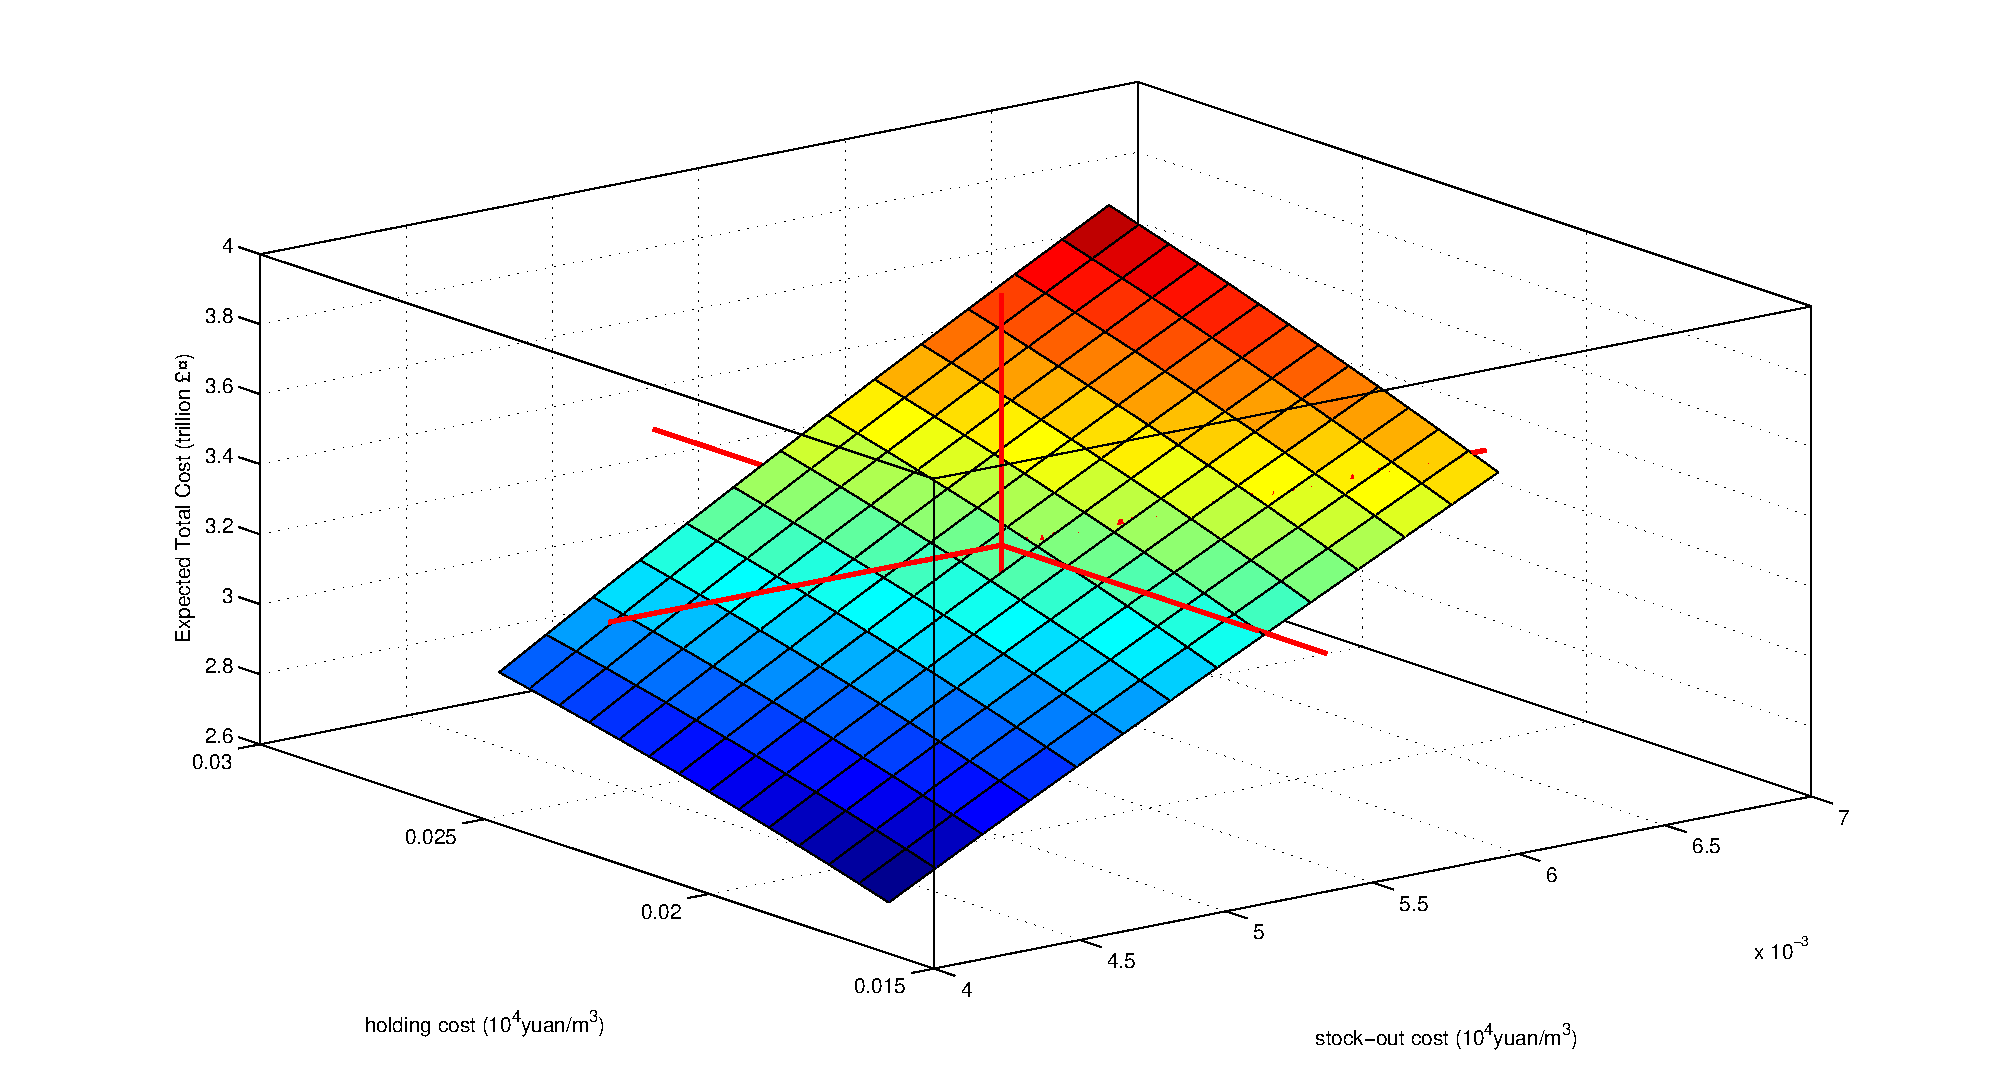
\includegraphics[width=15cm]{17444_figure_12}
\caption{\label{sensitivity2}Sensitivity result}
\end{figure}

\section{Strategy 3: Desalinization}
Desalinization refers to the process that removes some amount of salt and other minerals from saline water, thus providing fresh water for human use and irrigation. Saline water is no doubt a huge source of water supply, so some costal regions have adopted desalination to solve water shortage, such as Saudi Arabia\cite{des}.\\
In China, Tianjin operates a desalinization plant to alleviate local critical water shortage. But desalination has not been extensively used across China. Here, we apply a NPV (net present value) method to examine the costs and benefits of establishing desalination plant and further decide whether to implement desalination.\\

\subsection{Potential Locations for Desalination}
Due to the nature of desalinization, target locations are restricted to costal regions. We first choose potential locations along cost according to the extent provinces are in water shortage. Based on our prediction in Section 2, we narrow down our target to 5 provinces that will be in severe water shortage in 2025, including Bejing, Tianjin, Shanghai, Jiangsu province and Shandong province(see \textbf{Figure \ref{figure6}}). Priority should be given to Jiangsu province with a predicted gap of 58.324 billion $m^{3}$.
\begin{figure}[htbp]
\centering
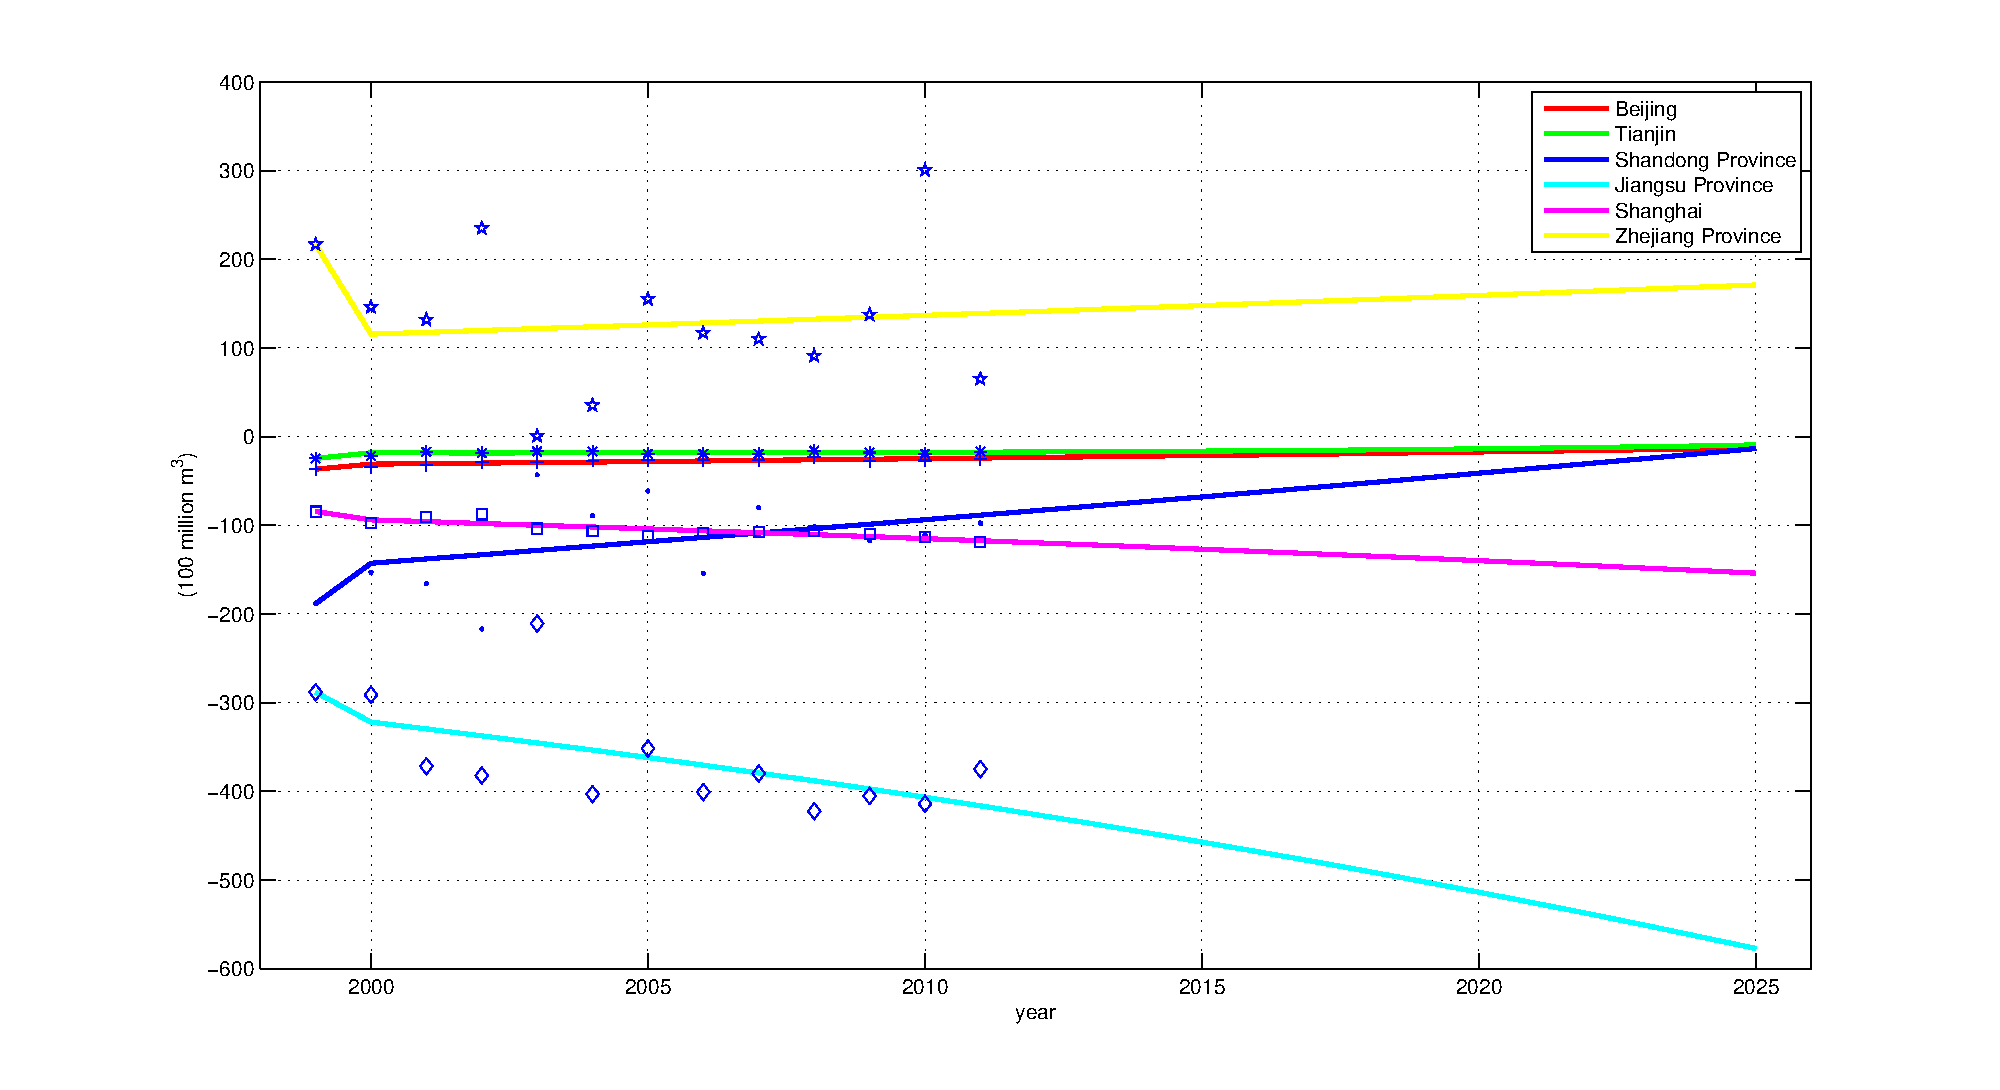
\includegraphics[width=15cm]{17444_figure_13}
\caption{\label{figure6}Comparison of water gaps in 6 provinces}
\end{figure}
Assume that it is feasible to establish desalination plants, both technologically and geologically, we next focus on its economic and social implications to see whether the potential social benefits exceed economic cost.

\subsection{Assumptions}
\begin{itemize}
\item \textbf{Desalination plant aims to fully satisfy the predicted water gap in each province.}
\item \textbf{No difference exists among desalination plants.} Each plant has the same capacity, initial investment,unit cost and operating cost.
\item \textbf{It takes 2 years to construct a plant,which is the average time needed.}
\item \textbf{We use contribution of water to local GDP as benefits of desalination plant.}Water is critical to agricultural production,industrial output and urban consumption, which further influence local GDP.
\end{itemize}

\subsection{Notations}
\begin{itemize}
  \item $CF_{i}(t)$: Cash flow of the $i^{th}$ province in period t.\\
  \item $V_{i}$:  Water contribution to GDP in province i.\\
  \item $GDP_{i}(t)$:  GDP for province i in period t.\\
  \item $S_{i}(t)$:   Water supply for province i in period t.\\
  \item $n$: The number of plants that each province need to establish to satisfy the water gap.\\
  \item $I$: Initial investment for each plant. We assume it to be 2 billion yuan. \\
  \item $OC$: Operating cost for each plant. We assume it to be 147 million yuan.
  \item $Ca$: Capacity for each plant. We assume it to be 5 billion yuan. \\
  \item $C$: Unit cost of dealing saline water for each plant. We assume it to be 1.5 million yuan. \\
  \item $r$: Discount rate. We set it to be 5.12\% \\
\end{itemize}
Note that the estimation are based on \textit{the prospectus for desalinization plant in Taoyuan, Taiwan}\cite{TW}.

\subsection{Cost-Benefit Analysis}
As we can see, costs include initial investment, operating cost per year and cost of dealing saline water per year, while benefit is defined as the contribution of water to local GDP. In each period, cash flow of establishing a desalination plant equals to:
$$CF_{i}(t)=V_{i}\rm{min}(GDP_{i}(t),S_{i}(t))-I\times n-OC\times n-Ca\times C\times n$$
where $V_{i}$, $GDP_{i}(t)$ and $S_{i}(t)$ are the average of the past three year's data for each province. Dividing water gap by the capacity, we can get the number of plant needed for each province, which is 1 for Beijing, 1 for Tianjin, 4 for Shanghai, 12 for Jiangsu and 1 for Shandong.\\
Taking discount rate into account, we get the calculation of NPV, which is:
$$ NPV_{i}=\sum_{t=0}^{12}\frac{CF_{i}(t)}{(1+r)^{t}} $$
where we use benchmark interest rate as our discount rate, which is 5.12\%. \\
The results show that it is profitable to establish desalination plant for each five province (see \textbf{Figure \ref{figure7}}). In particular, Jiangsu enjoy the highest profit implementing such a project, with a NPV of 24.46 trillion yuan.
\begin{figure}[htbp]
\centering
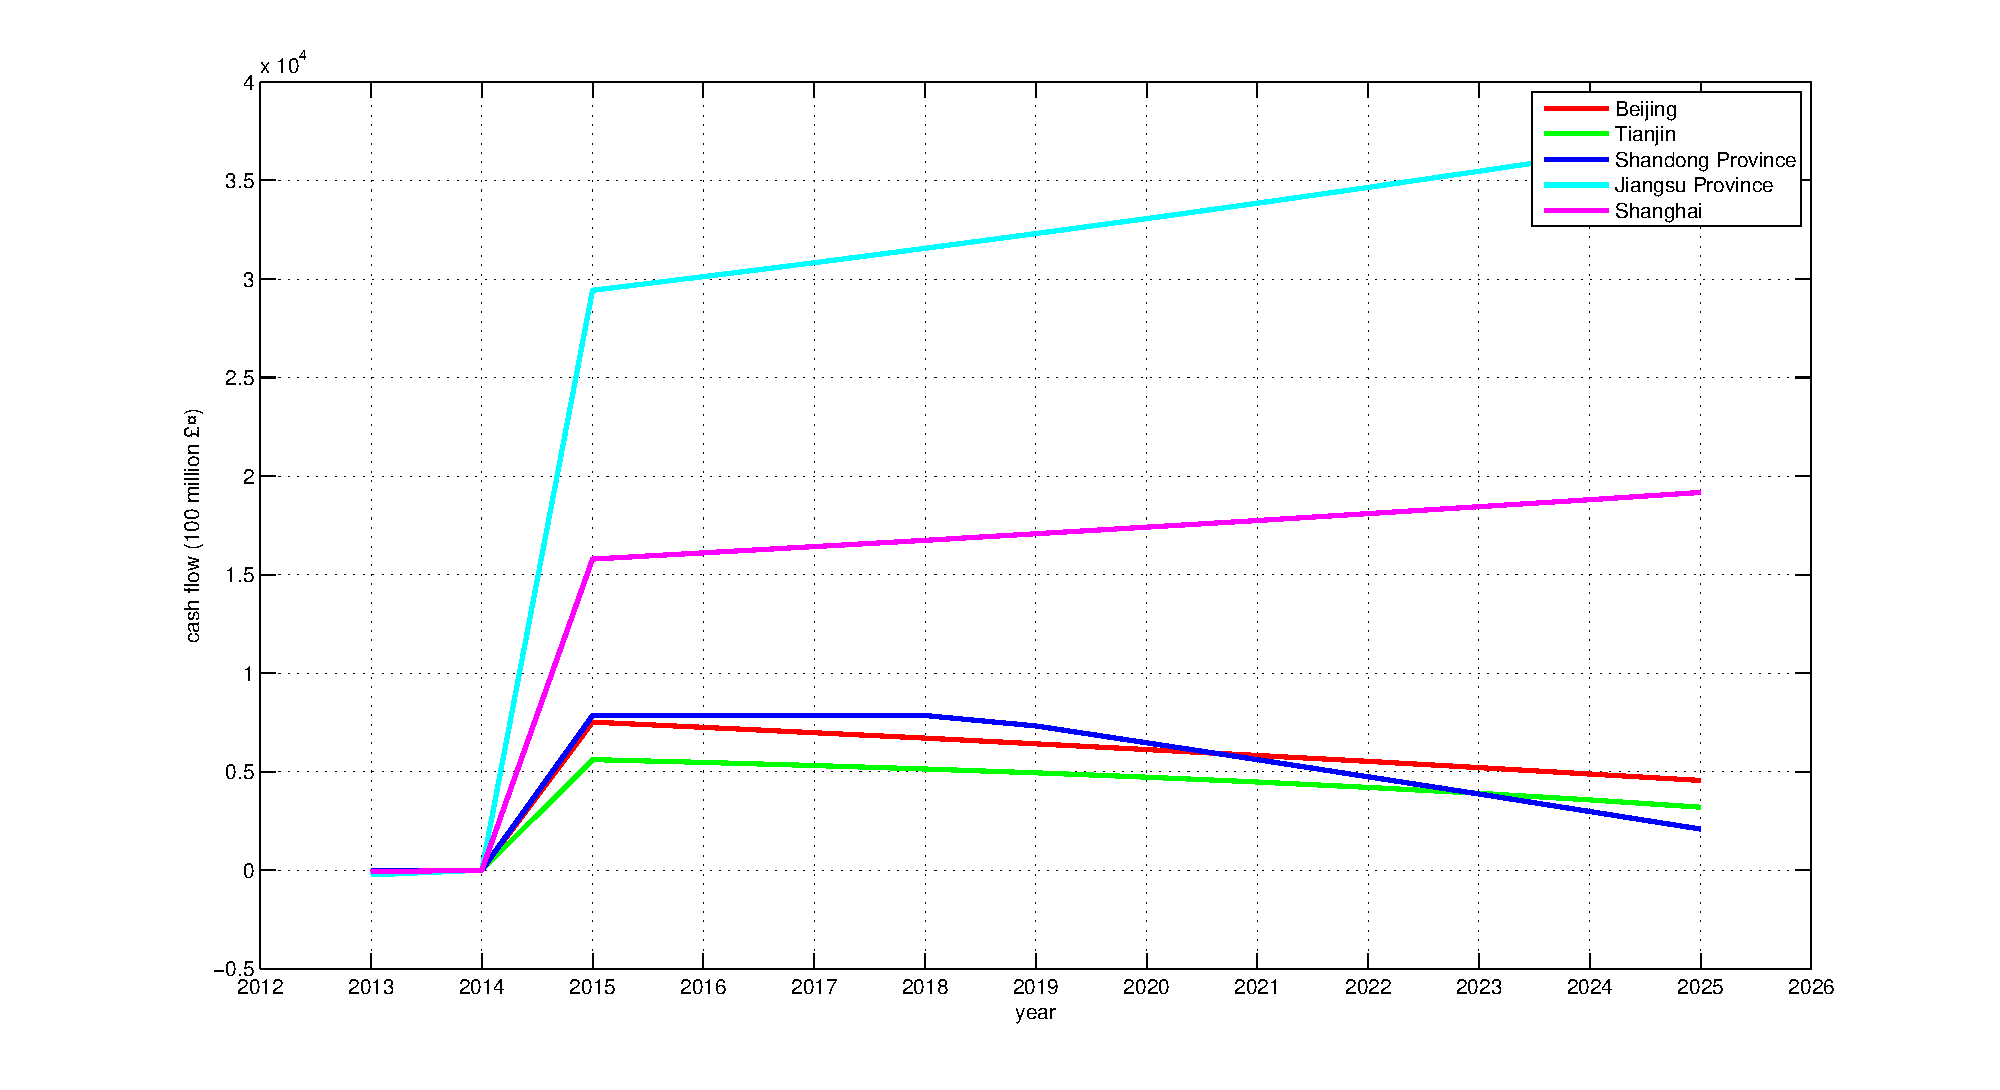
\includegraphics[width=15cm]{17444_figure_14}
\caption{\label{figure7}Cash flow of desalination plant in 6 provinces}
\end{figure}

\subsection{Strategy}
Without other strategies, we highly recommend costal regions to adopt desalination if it is technologically and geographically feasible to resolve the water shortage problem in 2025. However, it should be noted that capacity of existing plant in Tianjin is mostly hampered by poor local infrastructure and the low demand for drinking water\cite{Watts2011}. So when implementing desalination, the government should pay attention to better infrastructure construction and promote the desalinized drinking water.

\section{Strategy 4: Water Conservation}
Water conservation is as important as supply augmentation. In order to encourage citizens to conserve water and reduce waste, government has recently introduced such programs as increasing block tariffs, whose theoretical ground lies behind Ramsey Pricing. Through a case study of Shaanxi province, Liu and Gu\cite{Liu2009} found that increasing block tariffs helps save about 15 $m^{3}$ water per person per year. So the projection seems quite promising to resolve water shortage problem in the future. Here, we focus on how to determine optimal increasing block tariffs, including water price and block cutoff.\\
Central to Ramsey Pricing is that the price markup should be inverse to the price elasticity of demand multiplied by a constant lower than 1\cite{Ramsey1927}. Scholars have applied the theory into public service sectors, such as water sector, where government hopes to maximize social welfare rather than profit \cite{Boland1992}\cite{Henrique2011}. So, we also use Ramsey Pricing model to propose optimal water price for different income consumers.

\subsection{Assumptions}
\begin{itemize}
\item \textbf{We partition each province into agriculture sector, industry sector and urban sector and consider optimal pricing in each sector independently.} Agriculture, industry and urban consumption are three major drives for water use, of which the respective percentage is $61\%$ ,$24\%$ ,$13\%$.\cite{NBS}
\item \textbf{Based on different income owned by consumers in each sector, we partition each sector into low income, medium income and high income.} Three blocks are used extensively both in theory and practice, because too many blocks are difficult to implement while too few blocks are ineffective in water conservation \cite{Ma2008}.
\item \textbf{Demand in each block is endogenous, which can be adjusted by water price.} Classic economic theory states that price is a strong tool to affect demand.
\item \textbf{We consider government as the water supplier firm and the marginal cost and fixed cost remain the same for different groups in each sector.}
\item \textbf{The government only require that total revenue equal to total cost.} Unlike corporations, water supplier firm pays more attention to social welfare. Even it does generate profit, the profit is usually quite low \cite{Pushpangdadan1998}.
\item \textbf{Pricing strategy is the same for three sectors.} For simplicity, the model presented below describes the strategy in one sector and can be applied in the other two.
\end{itemize}

\subsection{Notations}
\begin{itemize}
 \item $Q_{i}$: Demand for different income groups, where i can be low, medium or high. \\
 \item   $P_{i}$: Price for different income groups, where i can be low, medium or high \\
 \item   $\varepsilon_{i}$: Demand elasticity for different income groups, where i can be low, medium or high. \\
 \item   $C_{i}$: Intercept in demand equation for different income groups, where i can be low, medium or high. \\
 \item  $TC$: Total cost faced by the government. \\
 \item   $MC$:  marginal cost faced by the government, which remains the same in each sector. \\
 \item $F$: Fixed cost faced by the government, which remains the same in each sector.\\
 \item $TR$:  Total revenue earned by the government. \\
 \item $SW_{i}$:  Marginal social welfare for different income groups, where i can be low, medium or high.\\
 \item   $SW$: Social welfare for each sector. \\
\end{itemize}

\subsection{Model}
Bailey\cite{Bailey2004} used linear regression and double logarithm linear regression to describe the demand based on water price and found that the latter fits the data better. Align with Bailey's finding, we also adopt double logarithm linear regression, which can be written as:
\[
\ln Q_{L}=C_{L}+\varepsilon_{L}\ln P_{L}
\ln Q_{M}=C_{M}+\varepsilon_{M}\ln P_{M}
\ln Q_{L}=C_{H}+\varepsilon_{L}\ln P_{H}
\]
where $\varepsilon=\frac{dQ/Q}{dP/P}$, representing the demand elasticity for each group in one sector.\\
For the government, total cost can be written as:
\begin{equation}
TC=3F+MC(Q_{L}+Q_{M}+Q_{H})
\label{e11}
\end{equation}
and total revenue cost can be written as:
\begin{equation}
\begin{split}
TR=Q_{L}P_{L}+[Q_{L}P_{L}+(Q_{M}-Q_{L})P_{M}]\\
   +[Q_{L}P_{L}+(Q_{M}-Q_{L})P_{M}+(Q_{H}-Q_{M})P_{H}]\\
  =3Q_{L}P_{L}+2(Q_{M}-Q_{L})P_{M}+(Q_{H}-Q_{M})P_{H}
\end{split}
\label{e12}
\end{equation}
With one unit of water increased, consumers pay $P_{i}(Q_{i})$, and government pays $MC$. So the marginal social welfare can be written as:
$$
SW_{i}(Q_{i})=P_{i}(Q_{i})-MC
$$
We aim to determine an optimal demand to maximize total social welfare.The problem can be written as:
$$
\rm{max}\ SW=\sum[\int P_{i}(Q_{i})-MC]dQ_{i}
$$
To get optimal demand, we use the method of Lagrange multipliers to get optimal price for each consumption group first. The optimization problem above can be rewritten as:
\begin{equation}
\rm{max}\ L(Q_{i},\lambda)={\sum[\int P_{i}(Q_{i})-MC]dQ_{i}]+\lambda [\sum Q_{i}P_{i}(Q_{i})-TC-\Pi]}
\label{e13}
\end{equation}
Taking first-order derivation of equation \ref{e13} to zero, we get:
\[
\frac{P_{i}(Q_{i})-MC}{P_{i}(Q_{i})}=-\frac{\lambda}{1+\lambda}\frac{1}{\varepsilon_{i}}
\]
As a result, for each consumption group, we have:
\[
(1-\frac{MC}{P_{L}})\varepsilon_{L}=(1-\frac{MC}{P_{M}})\varepsilon_{M}=(1-\frac{MC}{P_{H}})\varepsilon_{H}
\]
Expressing $P_{M}$ and $P_{H}$ in terms of $P_{L}$, we get:
\begin{equation}
P_{M}=MC/(1-\frac{\varepsilon_{L}}{\varepsilon_{M}}\frac{P_{L}-MC}{P_{L}})
\label{e14}
\end{equation}
\begin{equation}
P_{H}=MC/(1-\frac{\varepsilon_{L}}{\varepsilon_{H}}\frac{P_{L}-MC}{P_{L}})
\label{e15}
\end{equation}
Plugging equation \ref{e14} and \ref{e15} into equation \ref{e11} and \ref{e12} and making total revenue equal to total cost, as we assumed, yields:
\begin{equation}
\begin{split}
3Q_{L}P_{L}+2(Q_{M}-Q_{L})MC/(1-\frac{\varepsilon_{L}}{\varepsilon_{M}}\frac{P_{L}-MC}{P_{L}})\\+(Q_{H}-Q_{M})MC/(1-\frac{\varepsilon_{L}}{\varepsilon_{H}}\frac{P_{L}-MC}{P_{L}})\\
=3F+MC(Q_{L}+Q_{M}+Q_{H})
\end{split}
\label{e16}
\end{equation}
where, $\ln Q_{i}=C_{i}+\varepsilon_{i}\ln P_{i}$. Solving the equation \ref{e16}, we can achieve the optimal price for different amount of water consumption and further the optimal demand, which can be used as cutoff for the increasing block tariffs.
\subsection{Example Analysis and Strategy}
Agricultural sector accounts for the most in the total use, but only recently do some provinces, such as Hunan province, begin to charge irrigation cost due to difficulties in implementing. So it might be premature to adopt increasing block tariffs in agricultural sector.\\
Introduced into urban sector recently, increasing block tariffs has received extensive discussion in China. Considering optimal strategy in urban sector, we apply an example analysis to test its validity.\\
Demand elasticity is roughly between -1 and 0 according to the basic microeconomic theory. Jia and Kang\cite{Jia2000} found that the figure is -0.346 in China. So we assign -0.4 to $\varepsilon_{M}$. In our model, low water consumption can be regarded as minimum requirement for water demand with a small elasticity of -0.7. The same logic applies to high water consumption group and we assign -0.1 to $\varepsilon_{H}$. For other parameters, we assign value subjectively (see \textbf{Table \ref{haha}}).\\
\begin{table}[htbp]
\centering
\caption{Notations}
\begin{tabular}{lll}
\toprule
$\varepsilon_{L}=-0.7$ & $\varepsilon_{M}=-0.4$ & $\varepsilon_{H}=-0.1$\\
\hline
$C_{L}=2$ & $C_{M}=2.5$ & $C_{H}=3$  \\
\hline
$F=8$ & $MC=2$ \\
\bottomrule
\end{tabular}
\label{haha}
\end{table}
The results, which are summarized in table 5 and figure, show that when the consumption below about $10\ m^{3}/\rm{month}$, the optimal charge should be set at $2.07\ \rm{yuan}/m^{3}$. When the consumption between $10\ m^{3}/\rm{month}$ and $15\ m^{3}/\rm{month}$, the price should be $2.11\ \rm{yuan}/m^{3}$. When the consumption exceeds $15\ m^{3}/\rm{month}$. The results fit with common sense, but more thorough investigation should be taken to get more accurate value of parameters, which are essential for the final pricing policies.\\
\begin{table}[htbp]
\centering
\caption{Example Analysis: Optimal Pricing Strategy}
\begin{tabular}{llll}
\toprule
 & first block & second block & third block\\
\midrule
Q & 10.16 & 14.57 & 32.2 \\
\hline
P & 2.07 & 2.11 & 2.24 \\
\bottomrule
\end{tabular}
\label{ss}
\end{table}
Depending on the data provided by Liu and Gu\cite{Liu2009},we apply the results above to Xi'an city and obtain $17.8 m^{3}$ water saving per person per year, even more effective than the existing plan, indicating the strength of our method. However, thorough investigation should be taken to get more accurate estimations of parameters, which are essential for the final pricing policies, but we believe it is a strong tool to help government make wise decisions.
\begin{figure}[htbp]
\centering
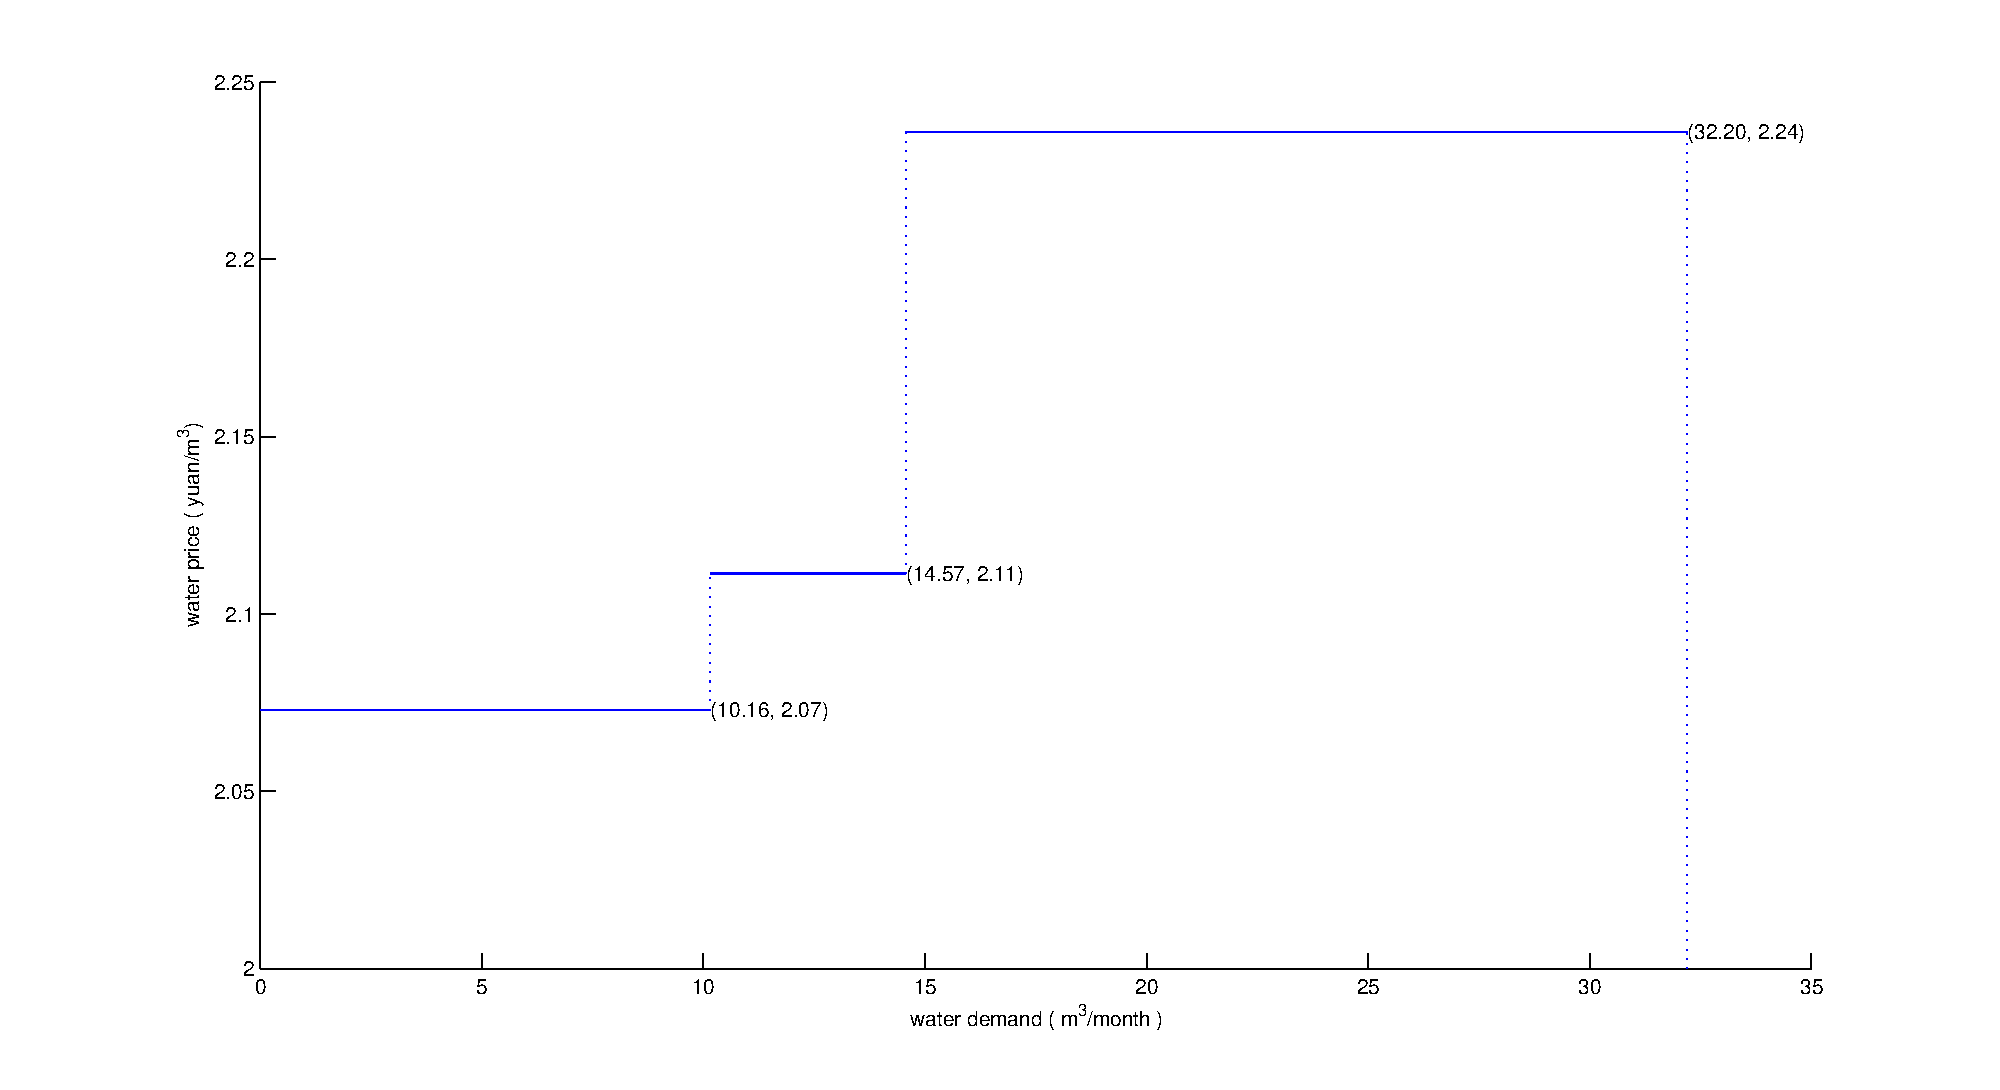
\includegraphics[width=12cm]{17444_figure_15}
\caption{\label{figure8}Example Analysis: Optimal Pricing Strategy}
\end{figure}

\section{A Comprehensive Strategy}
We now aim to synthesize four strategies discussed above into a comprehensive proposal for decision makers. We believe that each strategy has its pros and cons, which are summarized in \textbf{Figure \ref{sss}}, and the government should adjust measures according to local conditions when addressing water shortage.\\
\textbf{Water transfer} is advantageous in emergency situations, and is especially useful in dealing with uneven spatial distribution of water resource. However, water transfer project incurs a great amount of money and takes a long time to construct. \textbf{Water storage} is easy to implement in the sense that reservoirs are located near large rivers and enjoy easy access to water. The location of a reservoir, however, is also its limitation since it might also bring such negative impacts as too much pressure imposed on ecological environment. The strategy applies best when downstream demand is relatively stable, i.e., no major unexpected emergency arises. \textbf{Desalinization} produces water of higher quality, making it a powerful tool in regions that are lacking clean, usable water. While the strategy has almost unlimited source of water and can produce by-product such as salt, its cost relies heavily on related technology. Desalinization can only be applied in coastal regions now and we also recommend that it be adopted in developed cities first because it requires related infrastructure and market of drinking water. \textbf{Increasing block tariffs pricing} can be widely used in cities, with ease of implementation and relatively low cost. But the market response, reflected in demand reduction, might have time lag.
\begin{figure}[htbp]
\centering
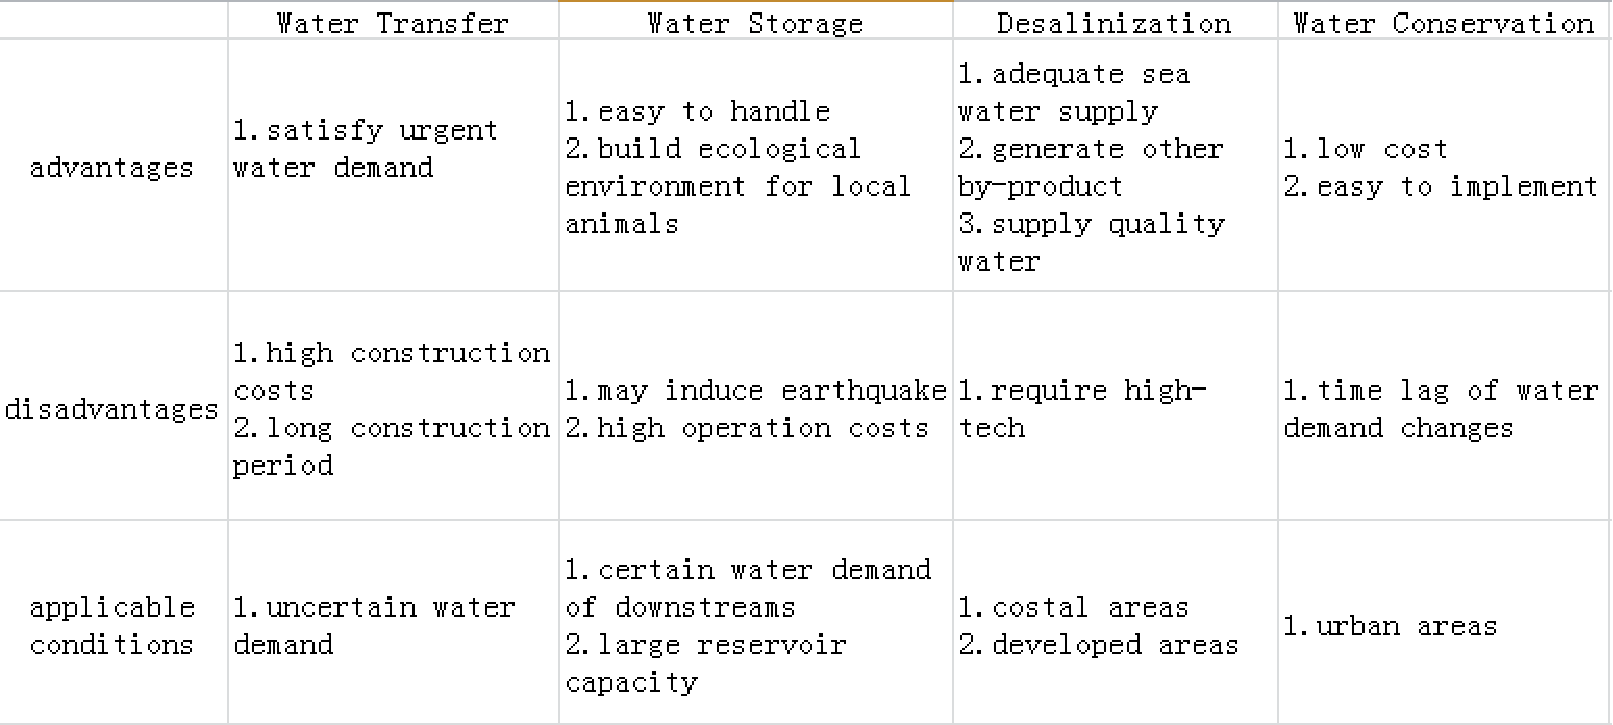
\includegraphics[width=12cm]{17444_figure_16}
\caption{\label{sss}Pros and cons of different models}
\end{figure}
Based on two criteria, which are inland area \emph{versus} coastal area and uncertain water demand \emph{versus} certain water demand, we can categorize four strategies into two dimension coordinate, as seen in \textbf{Figure \ref{dm}}. We define level of demand certainty as variations of historical data, which can be accessed by the department concerned.
\begin{figure}[htbp]
\centering
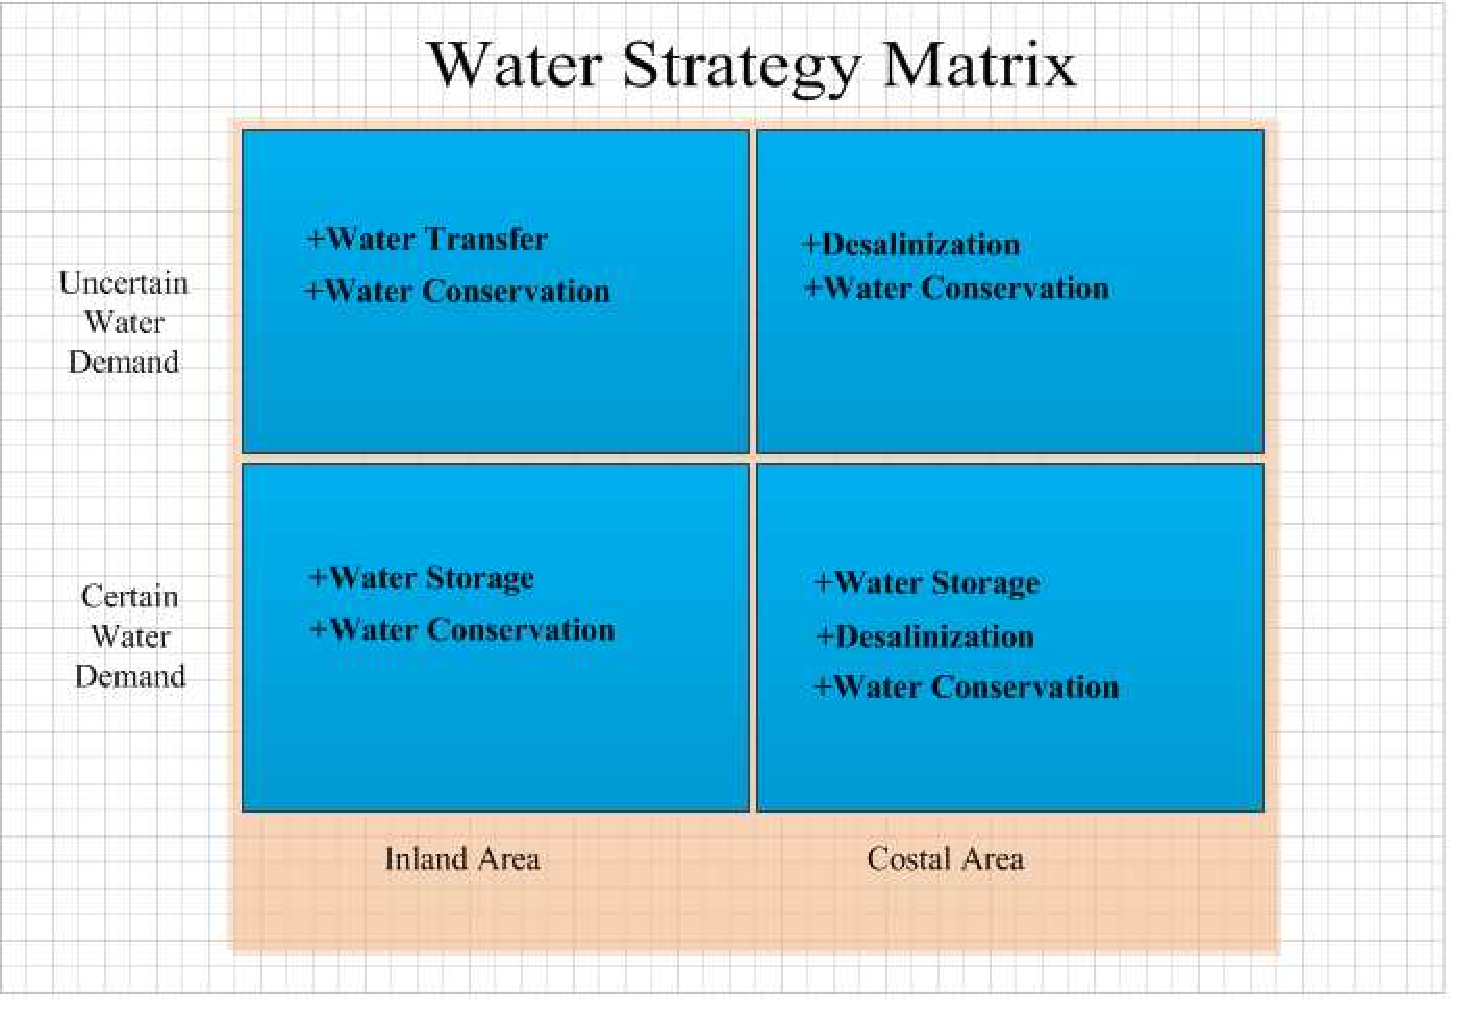
\includegraphics[width=12cm]{17444_figure_17}
\caption{\label{dm}Categorization of four strategies}
\end{figure}
Combined with our prediction of water gap, we propose 4 specific plans now to deal with the problem in 2025.
\begin{enumerate}
\item Priority should be given to \textbf{Jiangsu province} since it will suffer most from water shortage. Jiangsu is a relatively developed province, so we recommend \textbf{water storage, 5 desalinization plants and increasing block tariffs}. Many reservoirs are located in Jiangsu, department concerned should pay attention to make stock policy based on our news-vendor model. 5 desalinization plants are suitable considering other strategies to cut water gap. In fact, IBT has been introduced into Nanjing city and Nantong city, and we highly recommend that it be promoted across the province by using our model provided. Investigation should be careful carried out to estimate parameters precisely.
\item Strategic position as it is in China, \textbf{Shanghai} also should be on top lists. Like Jiangsu province, Shanghai is a highly developed city along the coast and it is characteristic of scarcity of clean water, so we recommend \textbf{1 desalinization plant and increasing block tariffs} Considering high purchase power of consumers in Shanghai, we predict that the price set at large water consumption level should be higher than that in other cities, if our model is used correctly.
\item \textbf{Henan} is representative of inland area which mainly depends on agriculture, so we recommend \textbf{water storage} to solve the problem since the mainstream of Yellow river flows through He'nan province. Decisions should be carefully made on how much water needed to store for later gap. We believe our news-vendor model can help government make wise decision.
\item For \textbf{Beijing, Tianjin and Shandong province}, we recommend \textbf{1 desalination in each region}, \textbf{water transfer from southern area and increasing block tariffs.} Three neighbouring provinces can generate great synergy.Typical of scarce water resource,northern China is direct beneficiary of water transfer project.
\end{enumerate}

\section{Conclusion}
\textbf{Q1: What is the estimated water demand and available water supply in 2025?}
Based on grey model, we predict that \textbf{15} provinces will be in short of water in 2025, most of which are located in northern China. Jiangsu province will be most endangered by water shortage,with a gap of 58.32 billion yuan.\\\\
\textbf{Q2: How to solve the foreseen gaps?}
Considering spatial distribution, we apply a transportation model to address water transfer.Partitioning the vast country into seven river basins and summing up water gaps of provinces belonging to the region, we find that the Haihe Basin and the Yellow River Basin will be short of water in 2025. Assuming transport cost is proportional to distance, we get the optimal transfer strategy in which the Songliao Basin transfers water to the Haihe Basin and the Long River Basin to the Yellow River Basin, with a total cost of 14.88 yuan.\\
Considering temporal distribution, we apply a news-vendor model to address water storage. Regarding reservoirs as distributors who order water from its upstream to satisfy demands of its downstream,we aim to figure the optimal level of storage reservoirs need to prepare for future use. A case study of Three Gorges Reservoir reveals that $84.1 \rm{billion} m^{3}$ should be stored to meet the demand of its downstream, including Jiangsu, Anhui and Shanghai.\\
Considering supply augmentation,we apply a NPV method to determine whether to establish desalinization plant. We first narrow down the potential locations to 5 provinces that will suffer water shortage in 2025 along the coast and obtain the number of plants needed under the assumption that water gaps must be satisfied. Upon reasonable assumptions about costs and benefits, we find that NPV of the project in each province is positive, indicating that desalinization is economically and socially promising to solve the water shortage.\\
Considering demand constraint, we apply Ramsey pricing model to address water conservation. We aim to propose an optimal increasing block tariffs based on different water consumption. Through a relatively subjective example analysis, we demonstrate the validity of the model, but more precise estimation of parameters are needed to get the final result.\\\\
\textbf{Q3: How to implement four strategies properly?}Four strategies have their own pros and cons, so we should take measures according to local conditions. In order to provide a succinct and clear guide for government to make decisions, we categorized strategies according to two criteria, which are inland area versus coastal area and uncertain water demand versus certain water demand. Desalination and increasing block tariffs should be adopted in cities rather than rural areas.\\
For those which will face water shortage in 2025, we propose detailed plans. More specifically, we recommend Jiangsu adopt water storage, desalination and increasing block tariffs, Shanghai adopt desalination and increasing block tariffs, Henan adopt water storage and Beijing, Tianjin, Shandong combined adopt desalination and water transfer.

\section{Strength and Weakness}
 One major problem facing us is the precision of data. Data from different resources follow different criteria, thus may present inconsistency overall. Also, although our data come from official sources like the National Bureau of Statistics of China, they are still subject to manipulation for many reason. Different interpretations of data, on the other hand, leads to different result.  Other data used for our parameter estimation, for example, per unit cost of water transportation, cost of building an desalinization plant and so forth is also hard to attain or estimate, these will greatly result in significant changes in final strategy should our estimation deviates from the intrinsic value.\\
However, to obtain the desired data is no easy job. These often require long-term surveys and study, as well as the assistance from expertise in related field. In several days, there is no way to accurately capture these data. Acknowledging this fact, we manage to build conceptual models with logical reasoning and mathematical calculation (The grey model is an exception. The reason for using a grey model is discussed in the section of prediction and an alternative conceptual model is also offered.), under the assumption that we have a precise data. This way, we are able to modify our final strategies as soon as we obtain more accurate data, say, from the government or other sources, without doing many burdensome repetitions.\\

\section{A Non-technical Position Paper to Governmental Leadership}
\noindent To Whom It May Concern,
\\\\
We are writing this position paper to suggest a best strategy which combines desalinization, conservation, movement and storage to help you tackle with projected water shortage facing China in 2025. \\\\
We estimate that situation will be quite severe in 2025. There will be about 15 provinces whose water needs can not be covered by local water supplies. Jiangsu province, in particular, will be faced with 58.32 billion $m^3$ of water shortage. Beijing, Shanghai and several other provinces also will be short of fresh water. \\\\
We suggest that in year 2025, the best water transfer strategy is to transport 12.32 billion $m^3$ of water from the Songliao Region to the Haihe Region, and 5.2 billion $m^3$ of water from the Long River to the Yellow River. On the other hand, our study on the Three Gorges Dam suggests that the Dam should store 84.1 billion $m^3$ of water from upstream to satisfy water needs in its downstream. For cities desalinization plants should be built in Shanghai, and several more in other provinces in need of water. The example of Shaanxi province tells us that an increasing block tariff pricing policy can well constrain water demands.\\\\
More specifically, in order to tackle with the severe water shortage in Jiangsu province, we suggest an increasing block tariff pricing policy combined with construction of 5 desalinization plants. Using more efficient storage strategy in water reservoirs can significantly generate stable water supplies to meet the demand in the province.\\\\
Our methodology combines four strategies together to deal with water shortage in a complicated environment in China. Jointly, these strategies covers demands of different degree of urgency, and different geographical distribution. We are confident that under various situation, our strategy will yield a optimal solution for you.\\\\
However, a major problem we encounter in our study is the precision and creditability of data. Since our models are conceptual ones using logical reasoning and mathematical computation, we are able to modify our final strategies as soon as we obtain more accurate data. Therefore, if you are interested in our study and provide us with field expertise and more credible results, we are more than happy to determine an even more detailed and effective strategy. We hope that with our joint effort, we can best alleviate water shortage and fight for a bright for the Country.\\\\
Best regards,\\\\
Team \#17444

\begin{thebibliography}{99}
\addcontentsline{toc}{section}{References}
\bibitem{Bailey2004}Bailey WR, Modeling domestic water tariffs, Proceedings of the 2004 Water Institute of Southern Africa (WISA) Biennial Conference
\bibitem{Boland1992}Boland JJ, Pricing urban water: Principles and compromises[J], Water Resource Update, 1992, 11(2):7-10
\bibitem{David1998}David Seckler, Upali Amarasinghe, David Molden, Radhika de Silva, and Randolph Barker, World Water Demand and Supply, 1990 to 2025: Scenarios and Issues, International Water Management Institute, 1998
\bibitem{Deng1989}Deng J., Introduction to grey system theory[J], The Journal of Grey System, 1989, 1:1-24
\bibitem{Dow2011}The Dow Chemical Company, China's Thirst for Water, 2011
\bibitem{Henrique2011}Henrique M and Catarina RP, Pricing for scarcity? An efficiency analysis of increasing block tariffs[J], Water Resource Research, 2011,47:1-11
\bibitem{Jia2000}Jia SF, Kang DY, Influence of water price rising on water demand in north Chian[J], Advances in Water Science, 2000, 11(1):49-53
\bibitem{Liu2009}Liu XJ, Gu Jinghua, Research on increasing block tariffs: A case study of Shanxi province[J]. Price: Theory and Practice, 2009, 2:22-23
\bibitem{Ma2008}Ma XW, Study on pricing strategy of increasing block tariffs[J], Science Technology and Engineering, 2008, 8(24): 1671-1819
\bibitem{NBS}The National Bureau of Statistics of China, Statistical Yearbook of China, 1999-2011
\bibitem{Oelkers2011}Oelkers2011 EH, Hering JG, Zhu C, Water: Is there a global crisis?[J], Elements, 2011,7(3):157-162
\bibitem{Pushpangdadan1998}Pushpangdadan K, Murugan G, Pricing with changing welfare criteria: An application of Ramsey-Wilson model to urban water supply, Working paper, 1998
\bibitem{Ramsey1927}Ramsey FP, A contribution to the theory of taxation[J], The Economic Journal, 1927, 37:47-61
\bibitem{TW}Water resource agency of Taiwan, the prospectus for desalinization plant in Taoyuan, Taiwan, 2008
\bibitem{Watts2011}Watts, Jonathan, Can the sea solve China��s water crisis?[J], The Guardian, 2011
\bibitem{des}Wikipedia, Desalination
\bibitem{Zhang2001}Zhang YJ and Liu QS, Evaluation and preference for water demand prediction method, China Water and Wastewater Journal, 2001, 1000-4602(2001)07-0027-03
\bibitem{Zhuo2011}Zhuo JW, Applications of MATLAB in mathematical modeling, Beihang University Press, 2011
\end{thebibliography}
